%%%%%%%%%%%%%%%%%%%%%%%%%%%%%%%%%%%%%%%%%%%%%%%%%%%%%%%%%%%%%%%%%%%%%%%%%%%%%%%

\chapter{CASE STUDY: HURRICANE BERYL}
\label{ch:beryl}

This chapter explores the results of implementing cold pool parameterization in the latest Brazilian numerical weather and climate prediction model, MONAN. It emphasizes the model's performance in predicting hurricane trajectory, intensity, and rainfall, using Hurricane Beryl as a case study, which occurred between June and July 2024 in the North Atlantic Basin. Following a brief introduction to the event, the chapter presents the results of the forecast and offers a direct comparison between ERA5 and MONAN. Finally, a discussion section will address the questions outlined previously in Table \ref{tab:questions}.
% VISTO

\section{Event description - hurricane Beryl}

Hurricane Beryl formed in the deep tropical Atlantic’s Main Development Region on June 28th, forming a tropical depression near 1200 UTC 28 June about 1200 nautical miles \footnote{In North American meteorology, it is common to use: pressure in millibars (mb), where 1 mb = 1 hPa; distance in nautical miles (nm), where 1 nm = 1.852 km; wind speed in knots (kt), where 1 kt = 1.852 km/h; and precipitation in inches (in), where 1 inch = 25.4 mm} east of Barbados, with a center at 1007 mb and wind speed of 30 kts. According to reports from the National Oceanic and Atmospheric Administration (NOAA), the storm rapidly intensified into a major hurricane, moving eastward and ultimately reaching Category 5 on the Saffir-Simpson Hurricane Wind Scale, making it the earliest Category 5 hurricane on record in the Atlantic Basin. Figure \ref{fig:hurricanepath} display all the trajectory computed with the best track dataset.

\begin{figure}[h!]
	\centering
	\caption{2024 Hurricane path according to best track analysis}
	\label{fig:hurricanepath}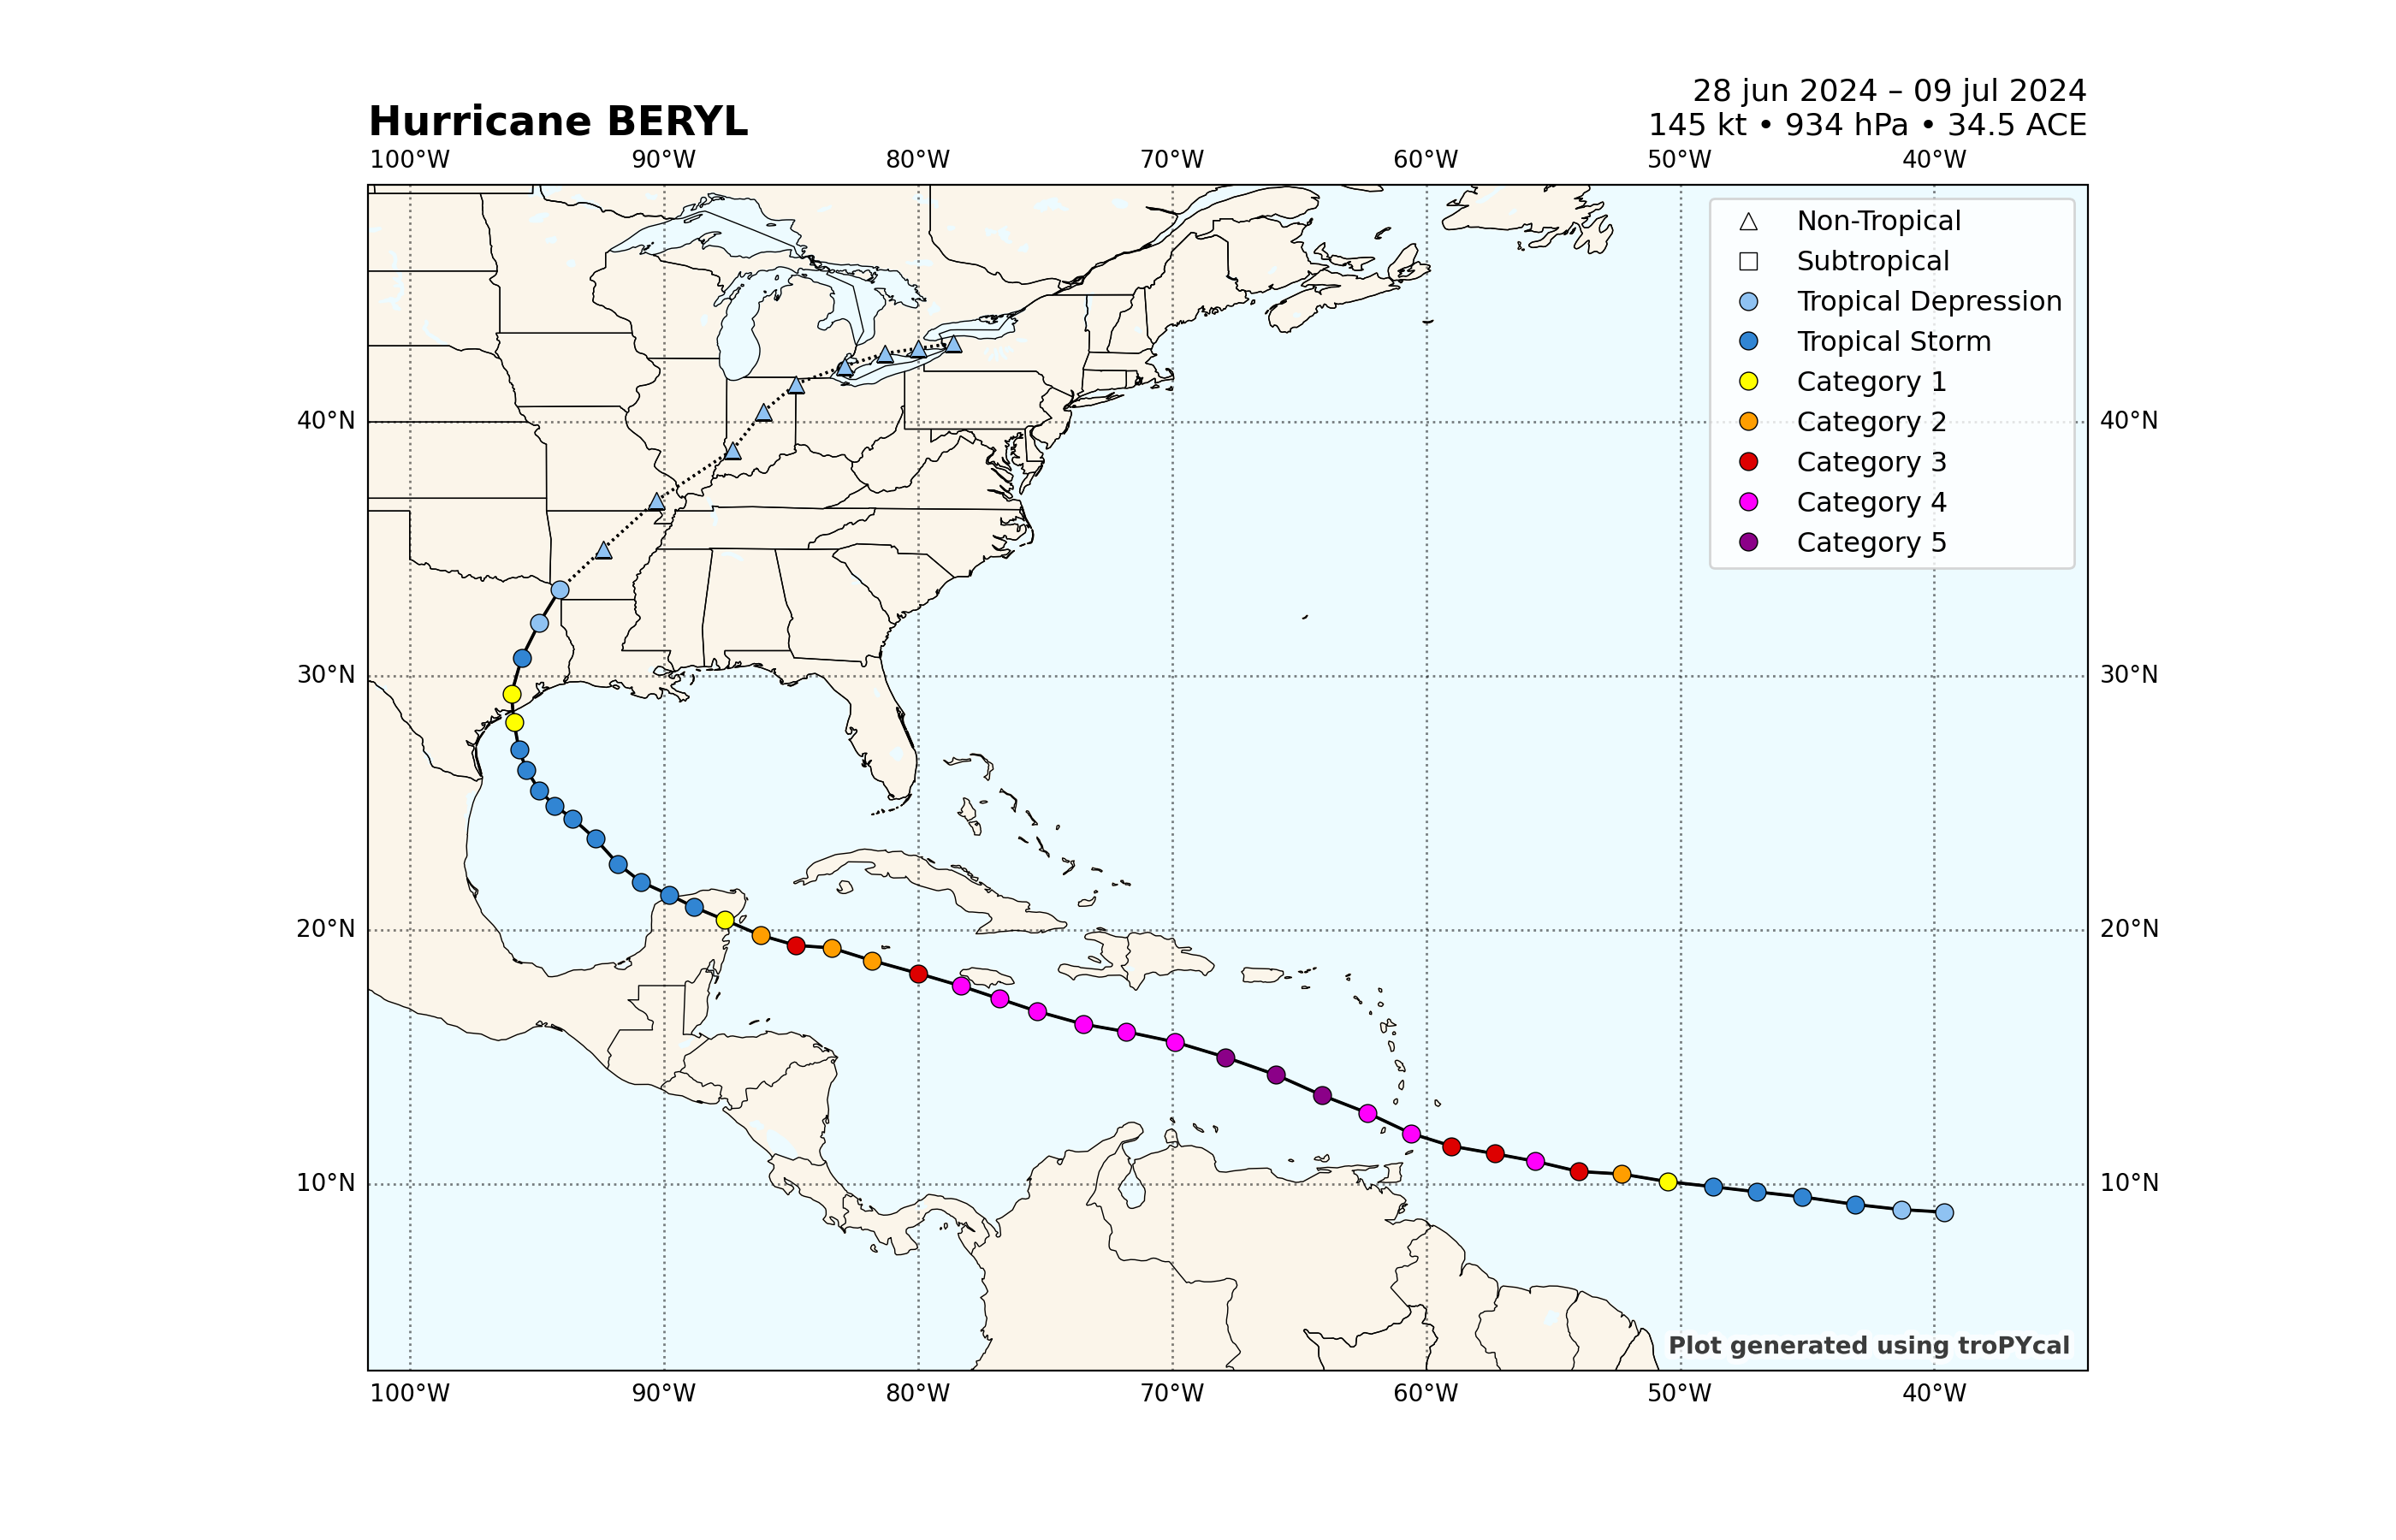
\includegraphics[width=\textwidth,height=\textheight,keepaspectratio]{docs/figuras/chapter5/beryl_2024.png}
	\centering
	Source: Made by the author (2025).
\end{figure}

It is important to note that the figure presented in the upper-right quadrant indicates critical meteorological parameters, including the peak wind speed recorded at 145 knots, the minimum mean sea level pressure of 934 hPa, and the Accumulated Cyclone Energy (ACE), which is quantified at 34.5. These values are derived directly from the best track dataset.

The first landfall of Hurricane Beryl occurred on the island of Carriacou in Grenada as a high-end Category 4 storm on July 1st, subsequently intensifying to a Category 5 in the Eastern Caribbean Sea. From a disaster perspective, the total damages in the Grenada Region are significant, with estimates of approximately US\$ 218.0 million, which accounts for about 16.5 percent of the GDP for 2023 \cite{gunasekera2024global}. Satellite images illustrating the hurricane's transition from Category 4 to Category 5, passing through the first landfall, are presented in Figure \ref{fig:HurricaneBerylBand13}.

\begin{figure}[h!]
	\centering
	\caption{Hurricane Beryl view from the GEOCOLOR composite (left) and Band 13 (right) when passing through the first landfall}
	
	\begin{minipage}{.48\textwidth}
		\centering
		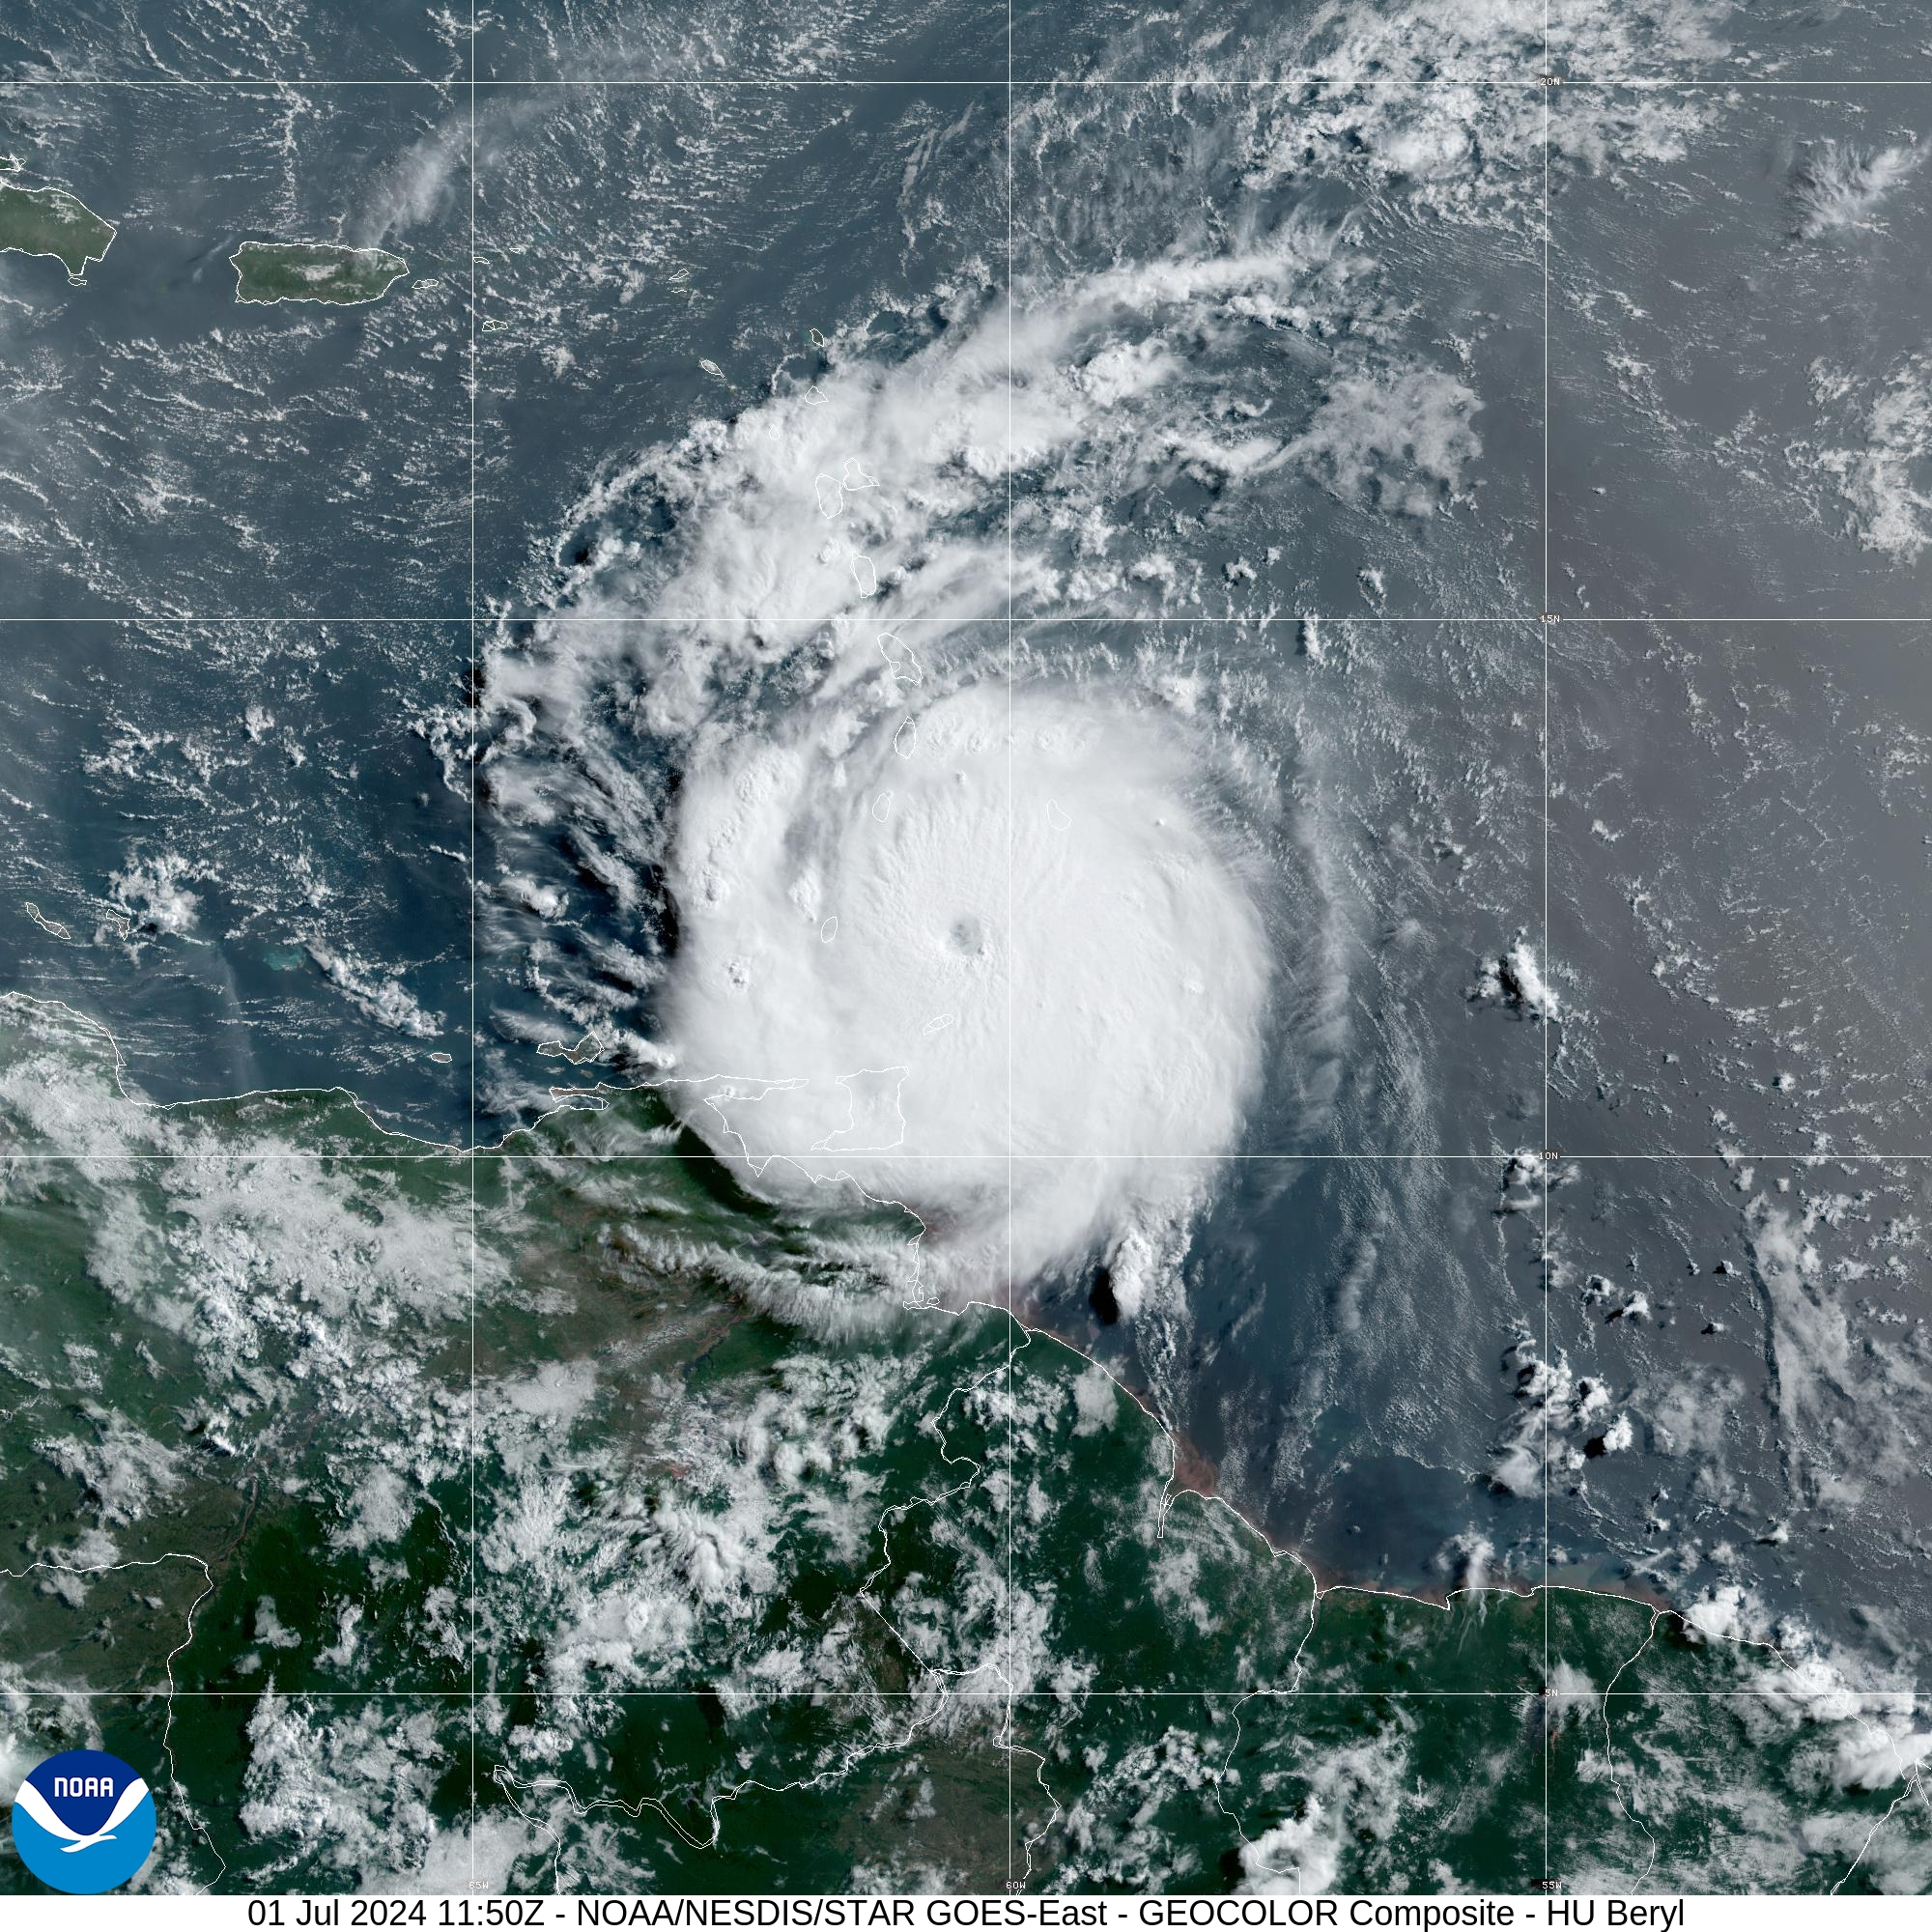
\includegraphics[width=\linewidth]{docs/figuras/chapter5/20241831150_GOES16-ABI-FL-GEOCOLOR-AL022024-2000x2000.jpg}
		\label{}
	\end{minipage}%
	\hfill
	\begin{minipage}{.48\textwidth}
		\centering
		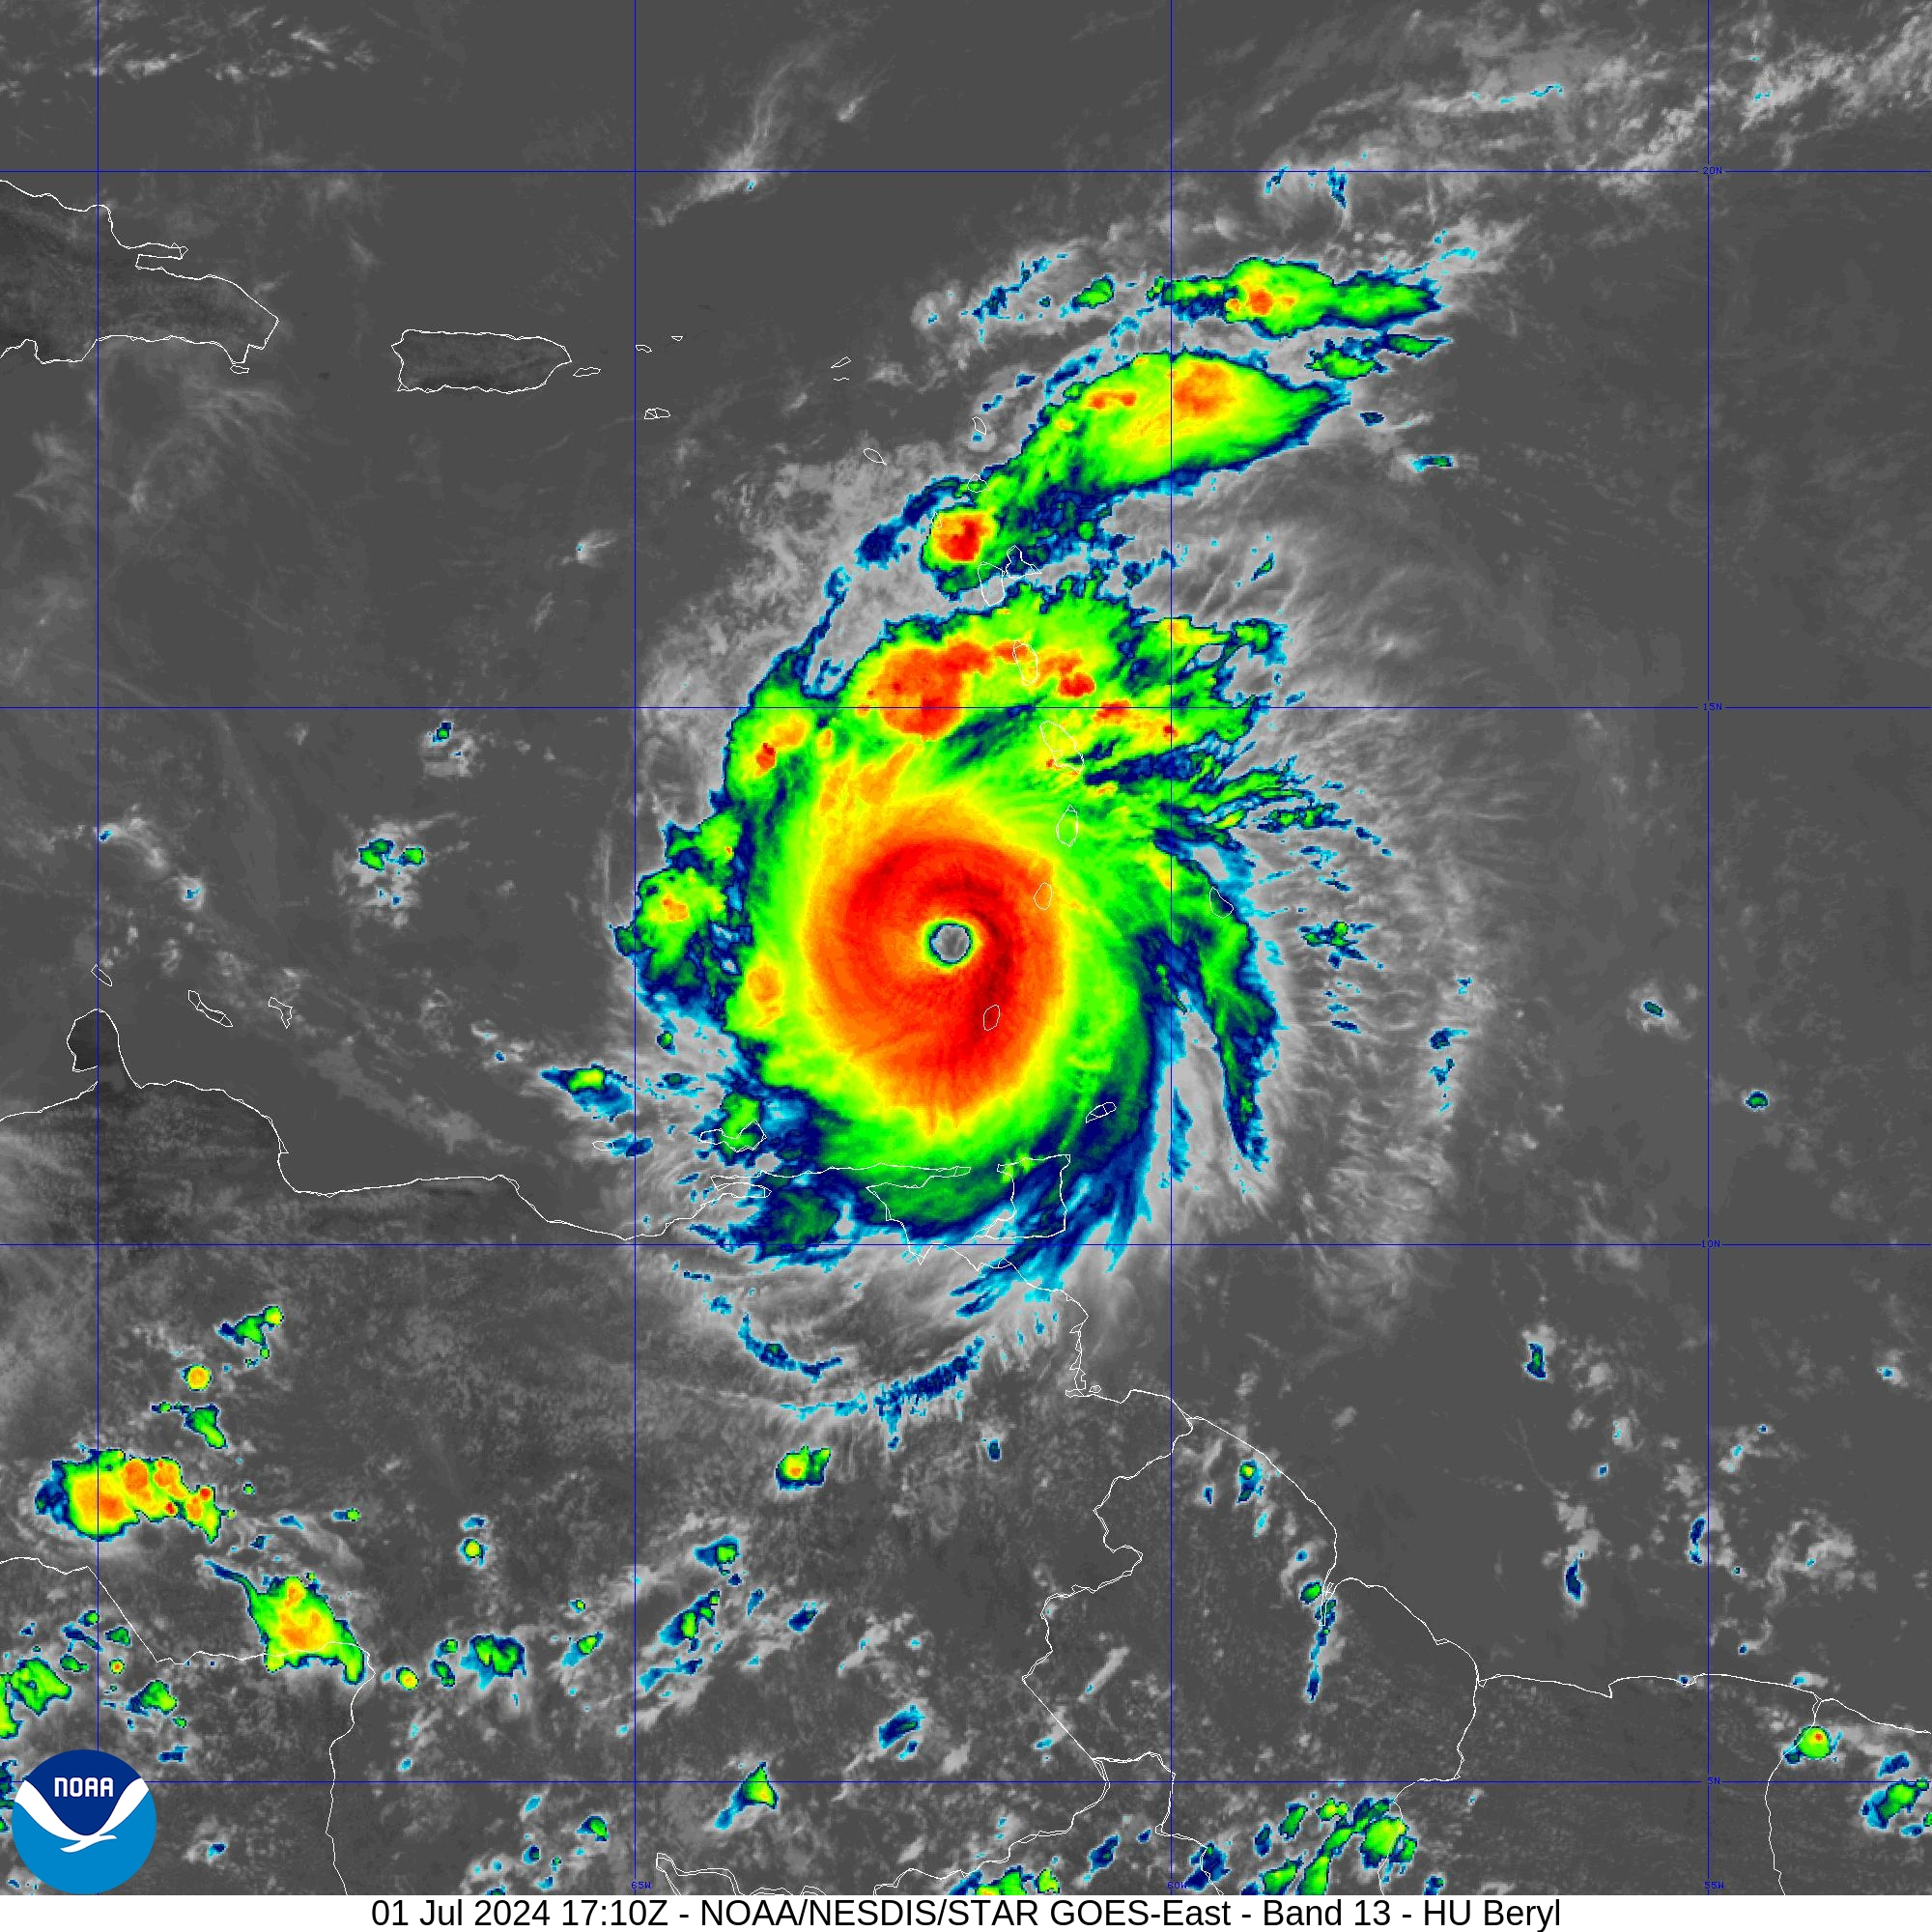
\includegraphics[width=\linewidth]{docs/figuras/chapter5/20241831710_GOES16-ABI-FL-13-AL022024-2000x2000.jpg}
		\label{fig:HurricaneBerylBand13}
	\end{minipage}
Source: \url{https://www.star.nesdis.noaa.gov/star/index.php.}
\end{figure}

At the passage through the Caribbean region, the rainfall was more intense in Jamaica, with widespread totals between 8 to 12 inches, and a peak of 13.62 inches observed at Knockpatrick in Manchester Parish, representing the highest storm-total rainfall reported.

The storm began to weaken before making a second landfall on the Yucatán Peninsula as a high-end Category 2 hurricane early on July 5th. Following its passage through the Peninsula, the hurricane continued to weaken while moving northwest, influenced by a large mid to upper-level trough of low pressure over the Central U.S., which eroded the robust ridge of high pressure over the Gulf of Mexico \cite{li2025generative}. The combination of increasing wind shear and dry air entrainment maintained a nearly steady state until dawn on July 7th. Later that morning, Hurricane Beryl progressed toward the Central Texas coast (northwest) as the mid to upper-level trough deepened to the north. An influx of moisture and decreased wind shear allowed the storm to become better organized, resulting in it being classified as a Category 1 hurricane by 11 PM CDT on July 7th (04:00 UTC on July 8th). A glimpse of this large scale environment is shown at Figure \ref{fig:mlsp}.

\begin{figure}[h!]
	\centering
	\caption{500 mb Geopotential Height and MSLP at July 8th, 00:00 UTC}
	\label{fig:mlsp}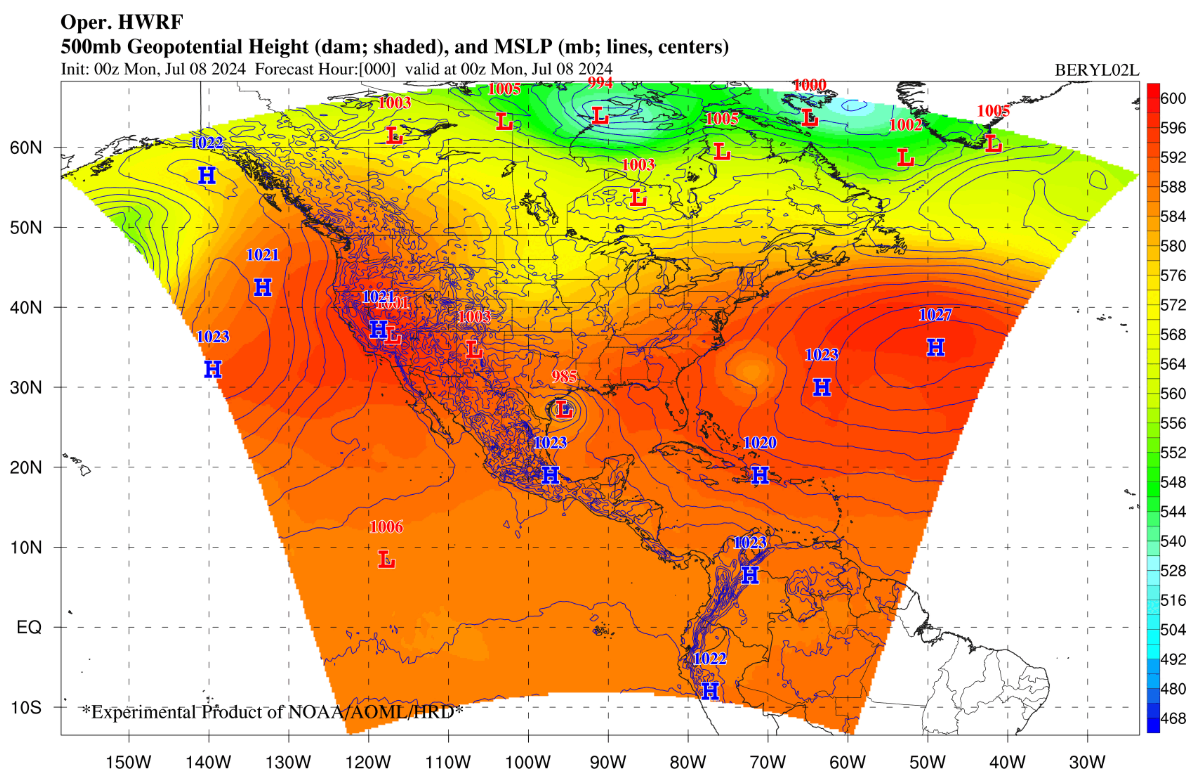
\includegraphics[width=\textwidth,height=\textheight,keepaspectratio]{docs/figuras/chapter5/beryl02l.png}
	\centering
	Source: \url{https://storm.aoml.noaa.gov/viewer/?projectName=BASIN}.
\end{figure}

At approximately 4 AM CDT on July 8th (09:00 UTC on July 8th), the hurricane made landfall near Matagorda along the Texas coast. Its maximum sustained winds were about 129 km/h (80 mph), and its minimum central pressure was 979 hPa. Figure 3 shows satellite and radar imagery capturing Hurricane Beryl's approach to the Texas coast.

\begin{figure}[h!]
	\centering
	\caption{HB view from NEXRAD (top) and GEOCOLOR composite (bottom) when reaching the Texas Coast.}
	\label{fig:nexradgeocolor}
	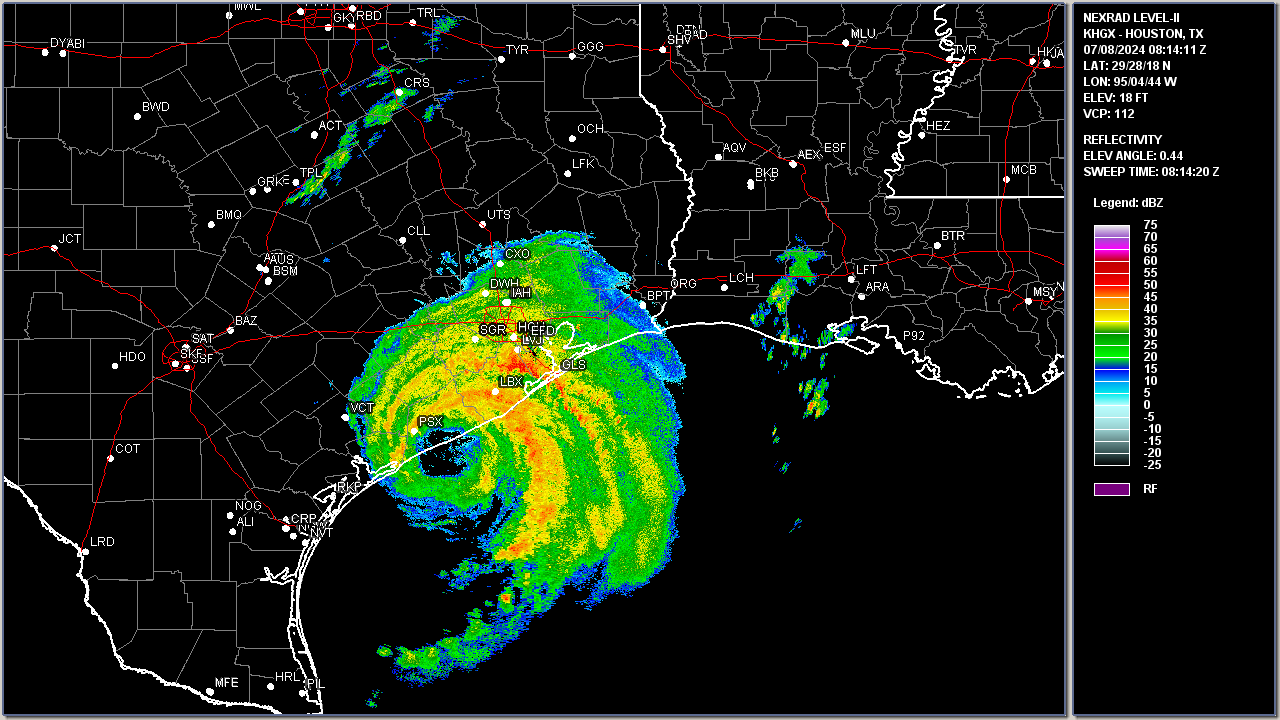
\includegraphics[width=0.8\textwidth]{docs/figuras/chapter5/20240708-0814Z-HGX.png}
	\vspace{3mm}
	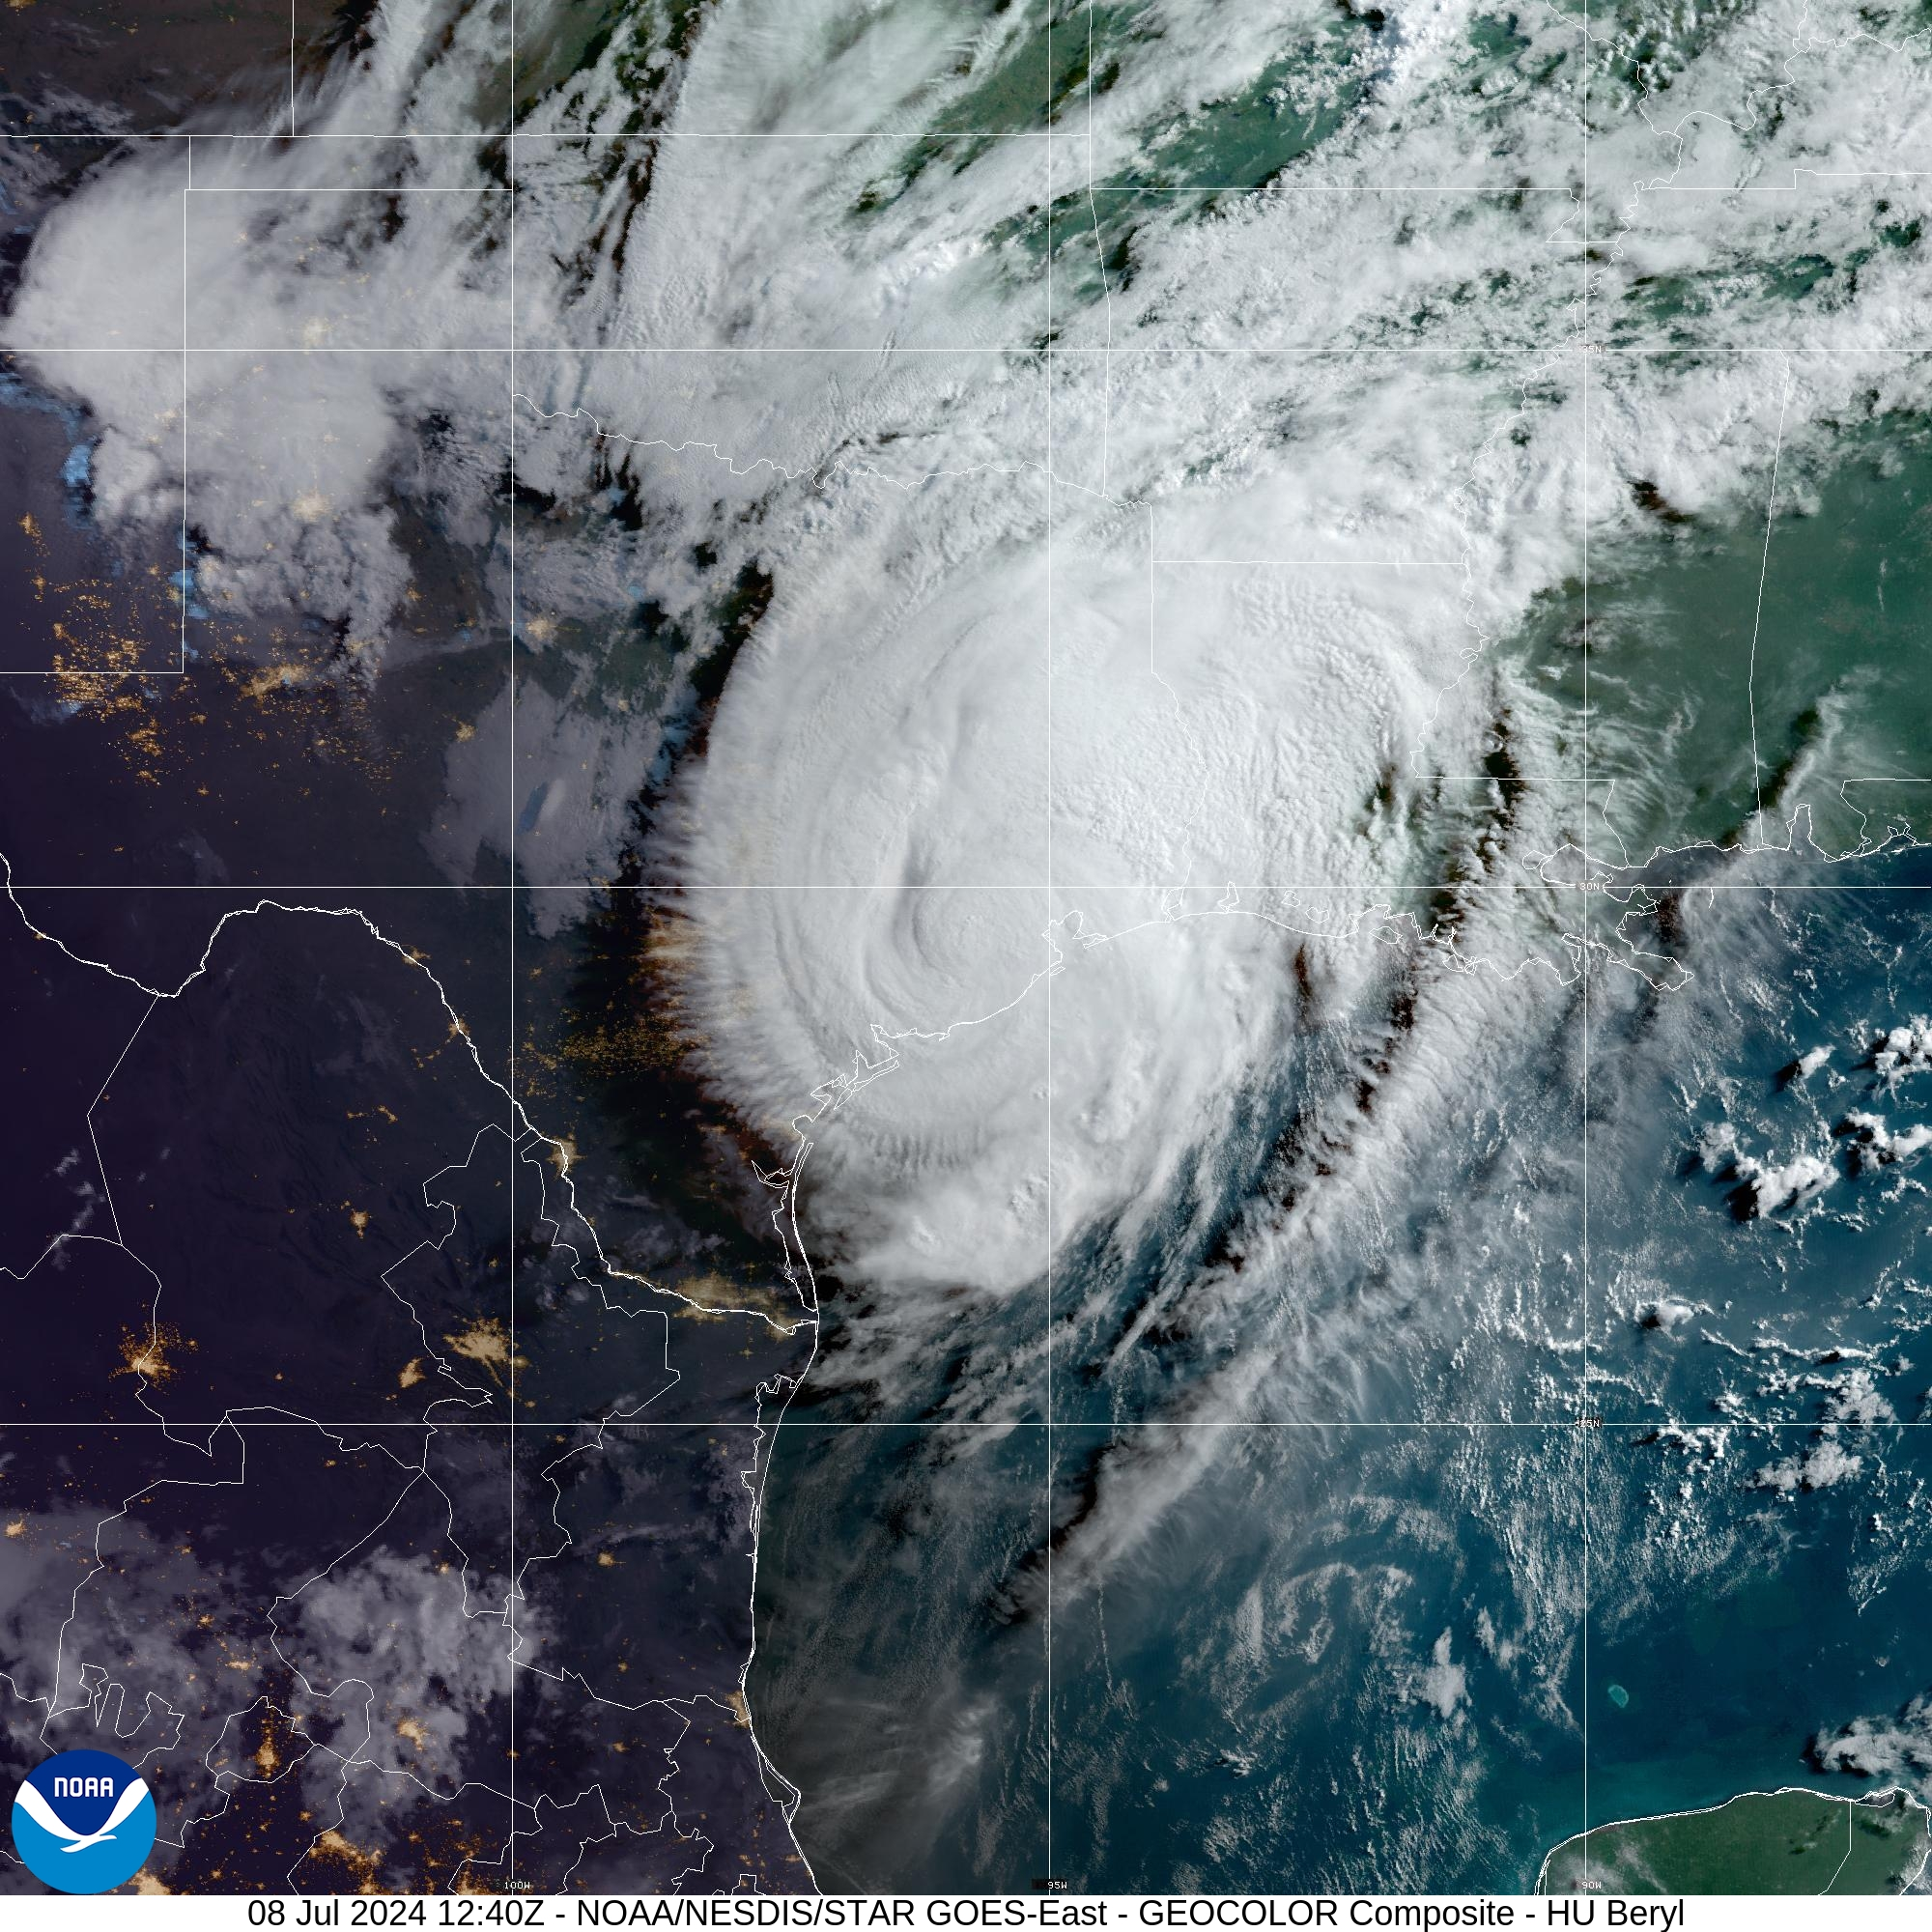
\includegraphics[width=0.6\textwidth]{docs/figuras/chapter5/20241901240_GOES16-ABI-FL-GEOCOLOR-AL022024-2000x2000.jpg}
	
	\centering
	Source: \url{https://www.star.nesdis.noaa.gov/star/index.php.}.
\end{figure}

Finally, the storm began to shift north-northeast, becoming a tropical storm by 10 AM CDT (15:00 UTC on July 8th). As it moved through the continental region, it weakened and transitioned to a tropical depression by 10 PM CDT (03:00 UTC on July 9th), just northwest of Shreveport, Louisiana.

Over the United States, the most intense rainfall occurred in the Houston metropolitan area in southeastern Texas, where widespread totals ranged from 8 to 12 inches, with local maxima of 14.99 inches in Thompsons and 14.88 inches at a HCFCD station in western Houston \cite{li2025generative}.

Based on this overview of the storm, Figure 4 has been created to illustrate the study area of interest, highlighting the significant landfalls made during its progression.

\begin{figure}[h!]
	\centering
	\caption{Spatial Domain of Hurricane Beryl's Development and Trajectory.}
	\label{fig:spatialdomainberyl}\includegraphics[width=\textwidth,height=\textheight,keepaspectratio]{docs/figuras/chapter5/map_with_cat_path.png}
	\centering
	Source: Made by the author (2025).
\end{figure}

The observational period for this study encompasses a six-day interval from 00 UTC on July 3 to 00 UTC on July 9, 2024, as illustrated by the gray bullet points in Figure \ref{fig:spatialdomainberyl}. Notably, this analysis will focus on a post-Category 5 storm. Whereas the system was active from June 28 to July 9, our analysis concentrates primarily on this specific timeframe. A sensitivity analysis regarding an earlier forecast of the observation period will be conducted and discussed in subsequent sections. This study encompasses significant geographical features, including the passage through Jamaica, which recorded the highest levels of rainfall in the Caribbean, the Yucatan landfall as denoted by the square E in Figure \ref{fig:spatialdomainberyl}, and the subsequent landfall in Texas, indicated by the square F in Figure \ref{fig:spatialdomainberyl}.

% ======================================================================================= %

\section{Results and analysis of hurricane Beryl}

In this section, we will present the results in alignment with the established workflow and engage in a discussion regarding the questions outlined in Table \ref{tab:questions}. The subsequent subsections will detail the trajectory, intensity, and rainfall analyses. To conclude, we will provide a summary discussion highlighting the key outcomes of the model and evaluating the overall performance of MONAN in comparison with ERA5 reanalysis.

By the workflow sequence, we will begin by addressing the selection process. Table~\ref{tab:experiments_long} illustrates all the experiments that were conducted.

\begin{table}[H]
	\centering
	\caption{All performed experiments}
	\label{tab:experiments_long}
	\renewcommand{\arraystretch}{1.2}
	\resizebox{\textwidth}{!}{
		\begin{tabular}{
				>{\centering\arraybackslash}m{3.5cm}
				>{\centering\arraybackslash}m{9cm}
				>{\centering\arraybackslash}m{4cm}
			}
			\toprule
			\textbf{Experiment} & \textbf{Description} & \textbf{ID} \\
			\midrule
			
			Cold Pool Effect 
			& Turn on and off the cold pool parameterization scheme 
			& \makecell[l]{CP-ON\\CP-OFF (Control)} \\
			\midrule
			
			Initial Condition Day 
			& Compares the effect of two initial conditions, June 29, July 2nd (noon), and July 3rd. Tested with 1st July 
			& \makecell[l]{CP-29\\CP-01\\CP-02T12\\CP-03} \\
			\midrule
			
			Cold Pool Lifetime 
			& Compares the effect of cold pool life time being 1h, 2h (default), 3h, and 6h 
			& \makecell[l]{CP-1H\\CP-2H\\CP-3H\\CP-6H} \\
			\midrule
			
			Maximum Downdraft Height 
			& Compares the effect of the maximum downdraft height, being 0.25, 0.35, and 0.50 
			& \makecell[l]{CP-D025\\CP-D035\\CP-D050} \\
			\midrule
			
			Resolution Experiment 
			& Evaluate the resolution effect on the results, degrading it into 60 km and enhancing it into 15 km 
			& \makecell[l]{CP-15km\\CP-30km (Control)\\CP-60km} \\
			\midrule
			
			Type of Initial Condition 
			& Changes the type of initial condition to be from the GFS model 
			& \makecell[l]{CP-ERA5 (Control) \\(CP-GFS)} \\
			\midrule
			
			Best Configuration Test 
			& A run with 2 changes inside the cold pool parameters 
			& \makecell[l]{CP-1HD050\\CP-1HD05015km} \\
			\bottomrule
		\end{tabular}
	}
	
	\vspace{2mm}
	{\centering Source: Made by the author (2025).\par}
\end{table}

The “ID” column serves as a reference for the names of the experiments. It is important to note that in the results, CP-ON represents the default configuration. In the sensitivity analyses conducted, the default values are specified in the labels. For instance, in the “Resolution Experiment,” the default configuration is set to a grid of 30 km (CP-30km), which is then changed to 60 km (CP-60km) and 15 km (CP-15km). To clarify, the following table emphasizes the default parameters:

\begin{table}[H]
	\centering
	\caption{Default values for the cold pool parameterization scheme}
	\label{tab:cp_def}
	\renewcommand{\arraystretch}{1.2}
	\resizebox{\textwidth}{!}{
		\begin{tabular}{
				>{\centering\arraybackslash}m{5.5cm} 
				>{\centering\arraybackslash}m{9cm}
			}
			\toprule
			\textbf{Parameter} & \textbf{Default value} \\
			\midrule
			Initial Condition Day & July 3rd, 2024 \\
			Cold Pool Lifetime & 2 h \\
			Maximum Downdraft Height & 0.35 \\
			Resolution Experiment & 30 km horizontal grid \\
			Type of initial condition & Coming from ERA5 \\
			\bottomrule
		\end{tabular}
	}
	
	\vspace{2mm}
	{\centering Source: Made by the author (2025).\par}
\end{table}




We investigate the impact of cold pools by enabling (CP-ON) and disabling (CP-OFF) the parameterization, with CP-OFF serving as the control experiment in this case. In the subsequent rows, we conducted a sensitivity analysis on the parameters within the parameterization. Now our control experiment is the CP-ON configuration, with the Table \ref{tab:cp_def} parameters. For the “Initial Condition Day” experiment, we varied the initial integration times: June 29 (00 UTC), 2024; July 1 (00 UTC), 2024; and July 2 (12 UTC), 2024 - comparing them with the default time. These periods were selected because they correspond to key moments in the storm’s evolution: shortly after HB was classified as a tropical storm, one day before it reached Category 5, and the day it reached Category 5, respectively.

The “Cold Pool Lifetime” was adjusted from the default to durations of 1 hour, 3 hours, and 6 hours. The height of the mass flux above the surface is described by a parabolic function, and the coefficient of this function can be manipulated to alter the maximum height, with lower (higher) values indicating proximity (distance) to the surface. The “Type of Initial Condition” was switched from ERA5 to GFS, both initialized on July 3 (00 UTC), 2024.

During the computation of the initial 13 experiments, we observed that setting the cold pool lifetime to 1 hour and adjusting the maximum downdraft height coefficient to 0.5 resulted in lower errors in the initial results. Consequently, we conducted the “Best Configuration Test” with these parameter adjustments and repeated this configuration at 15 km, bringing the total number of experiments to 15. The reference data here is the best track dataset, and hereafter this dataset will be referenced as “NOAA”. 

Keeping this in mind, Figure~\ref{fig:all_tracks_before} shows all the trajectories for the 15 experiments, plus ERA5 and the reference best-track dataset.

\begin{figure}[!htb]
    \centering
    \caption{Comparison of Storm Tracks Across All 15 Experiments} % Título acima da figura
    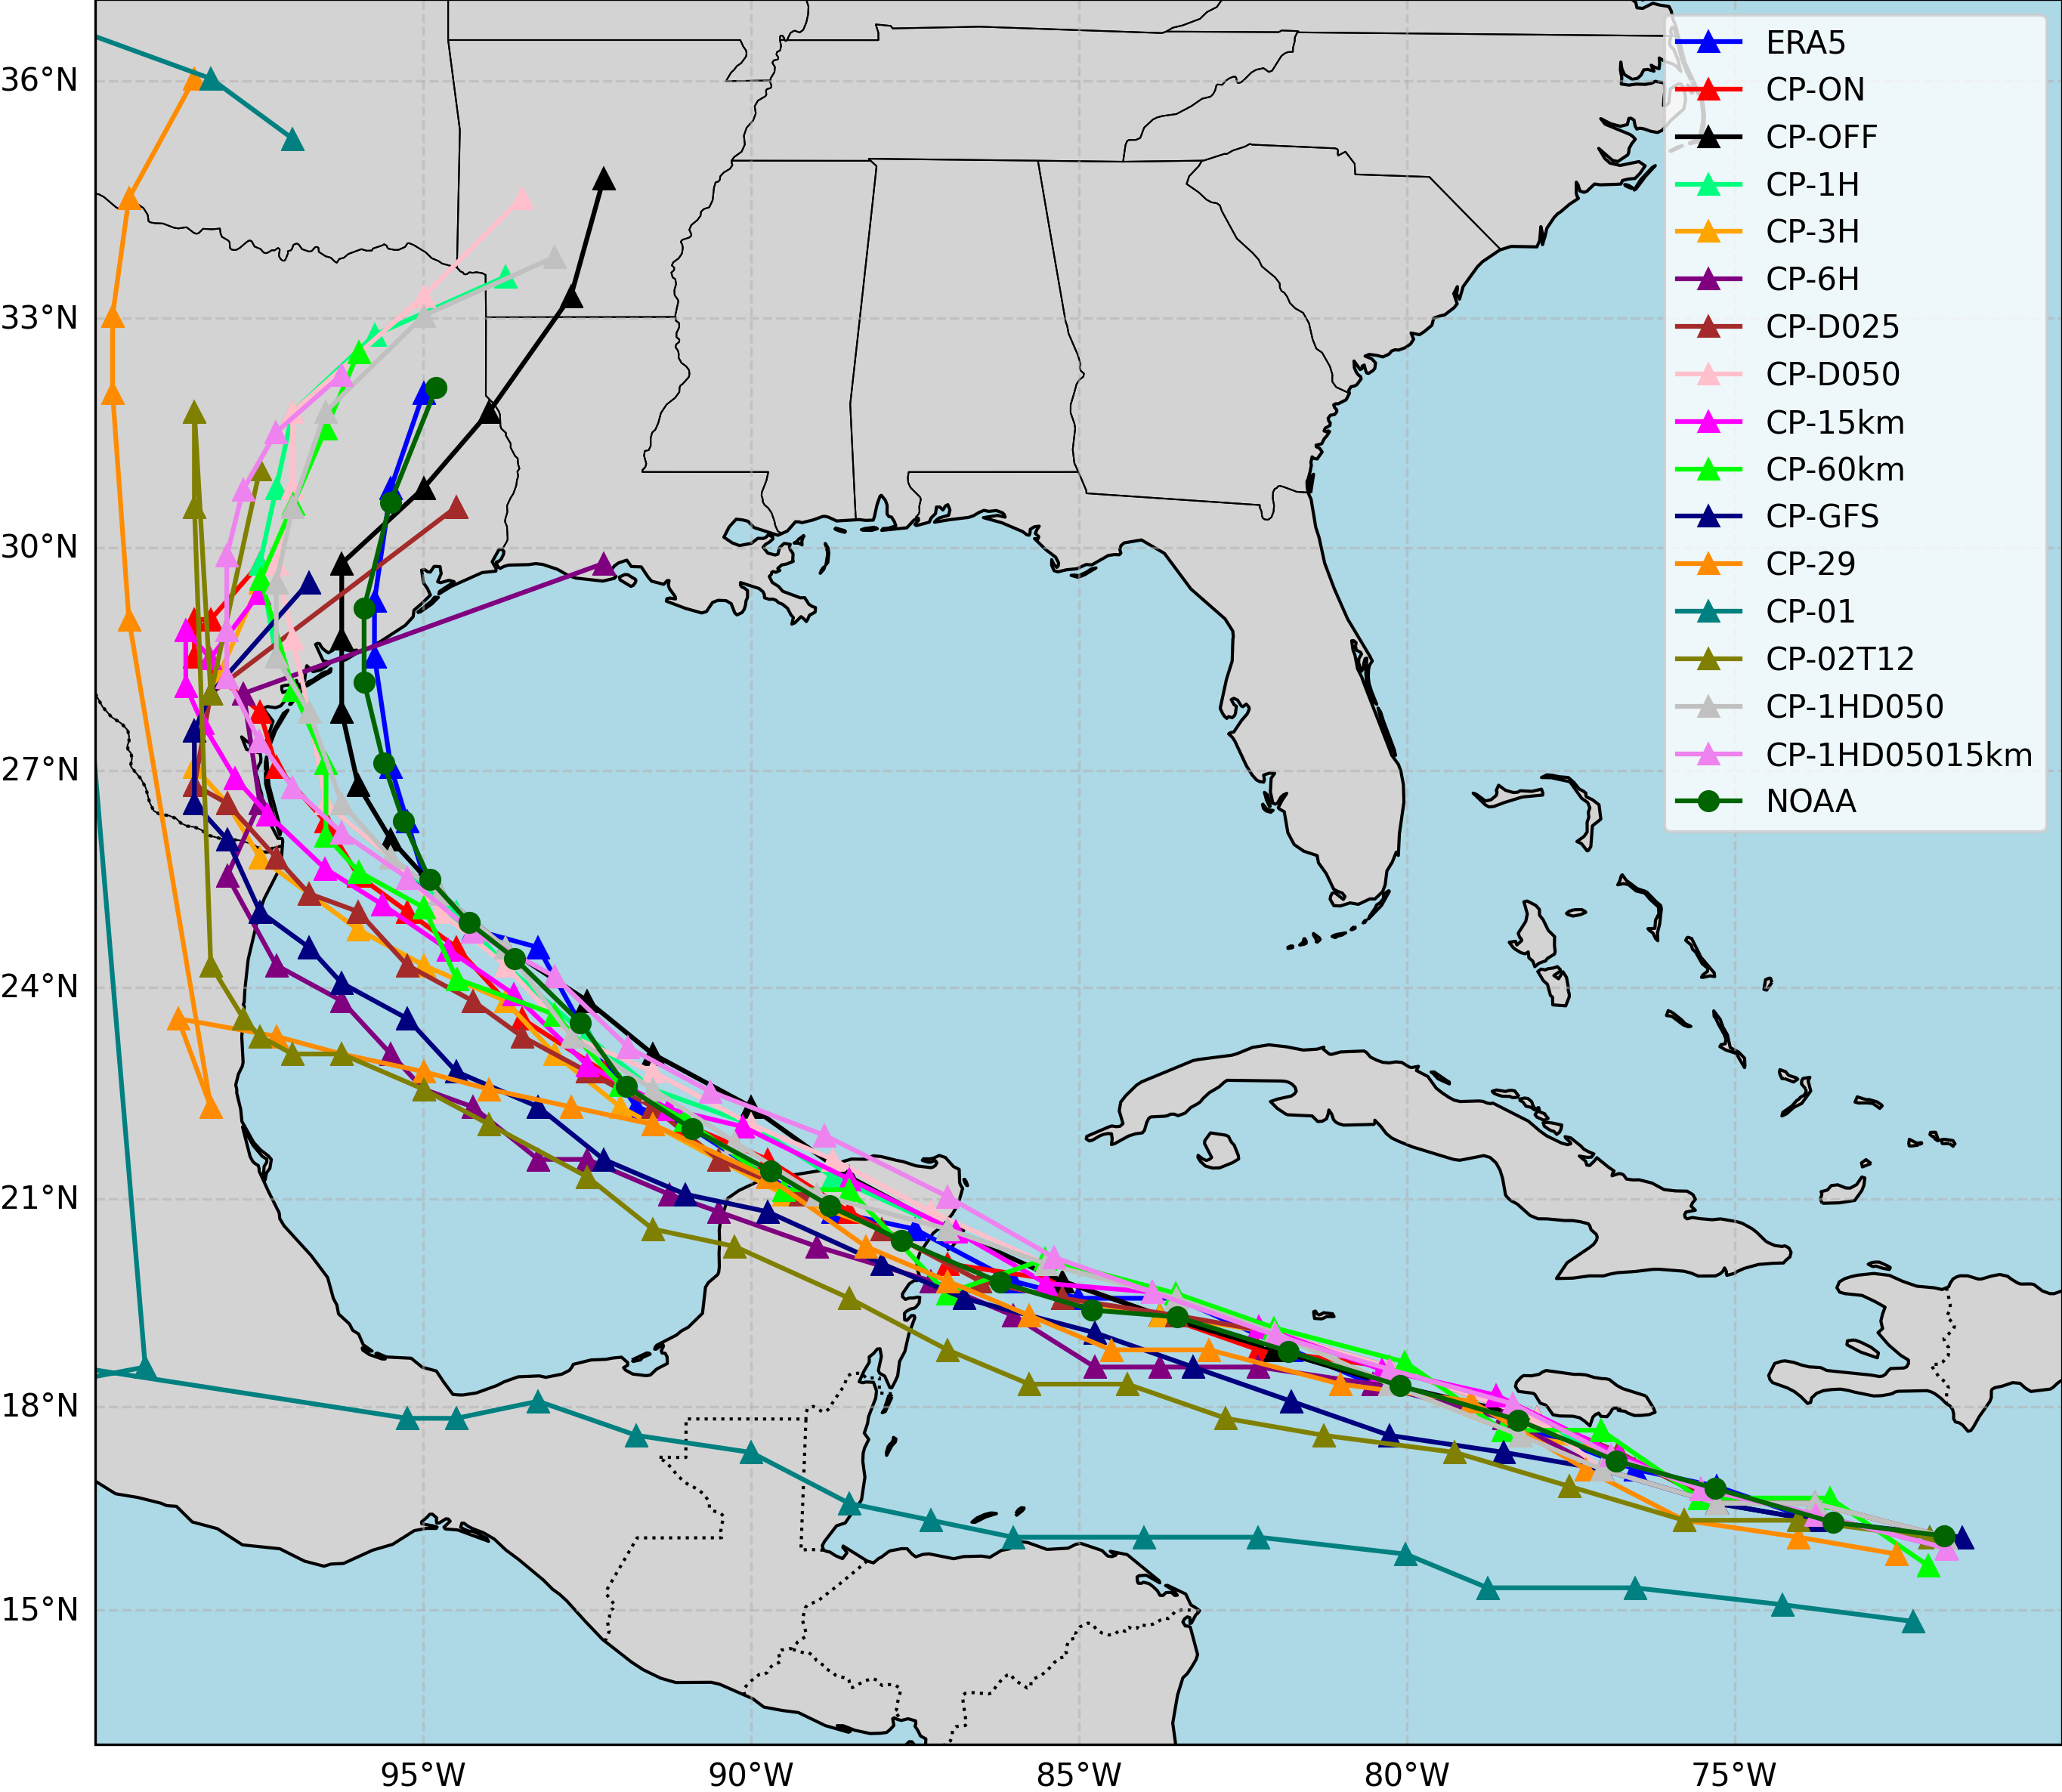
\includegraphics[width=\textwidth]{docs/figuras/chapter5/ALL_tracks_before_filter.png} % Substitua pelo caminho e extensão correta
    \vspace{0.5em}
    
    Source: Made by the author (2025). % Fonte abaixo da imagem
    \label{fig:all_tracks_before} % Label para referenciar no texto
\end{figure}

As one can see in Figure~\ref{fig:all_tracks_before}, the numerous experiments clutter the scene and make visual comparison difficult. But one could notice the deviation of CP-6H and CP-01, which could be candidates to be withdrawn. To better visualize the difference between the trajectories, the distance between each trajectory and the reference data (NOAA’s best track) was computed and shown in Figure~\ref{fig:panel_errors_before}.

\begin{figure}[!htb]
    \centering
    \caption{Errors (distance) between the trajectories} % Título acima da figura
    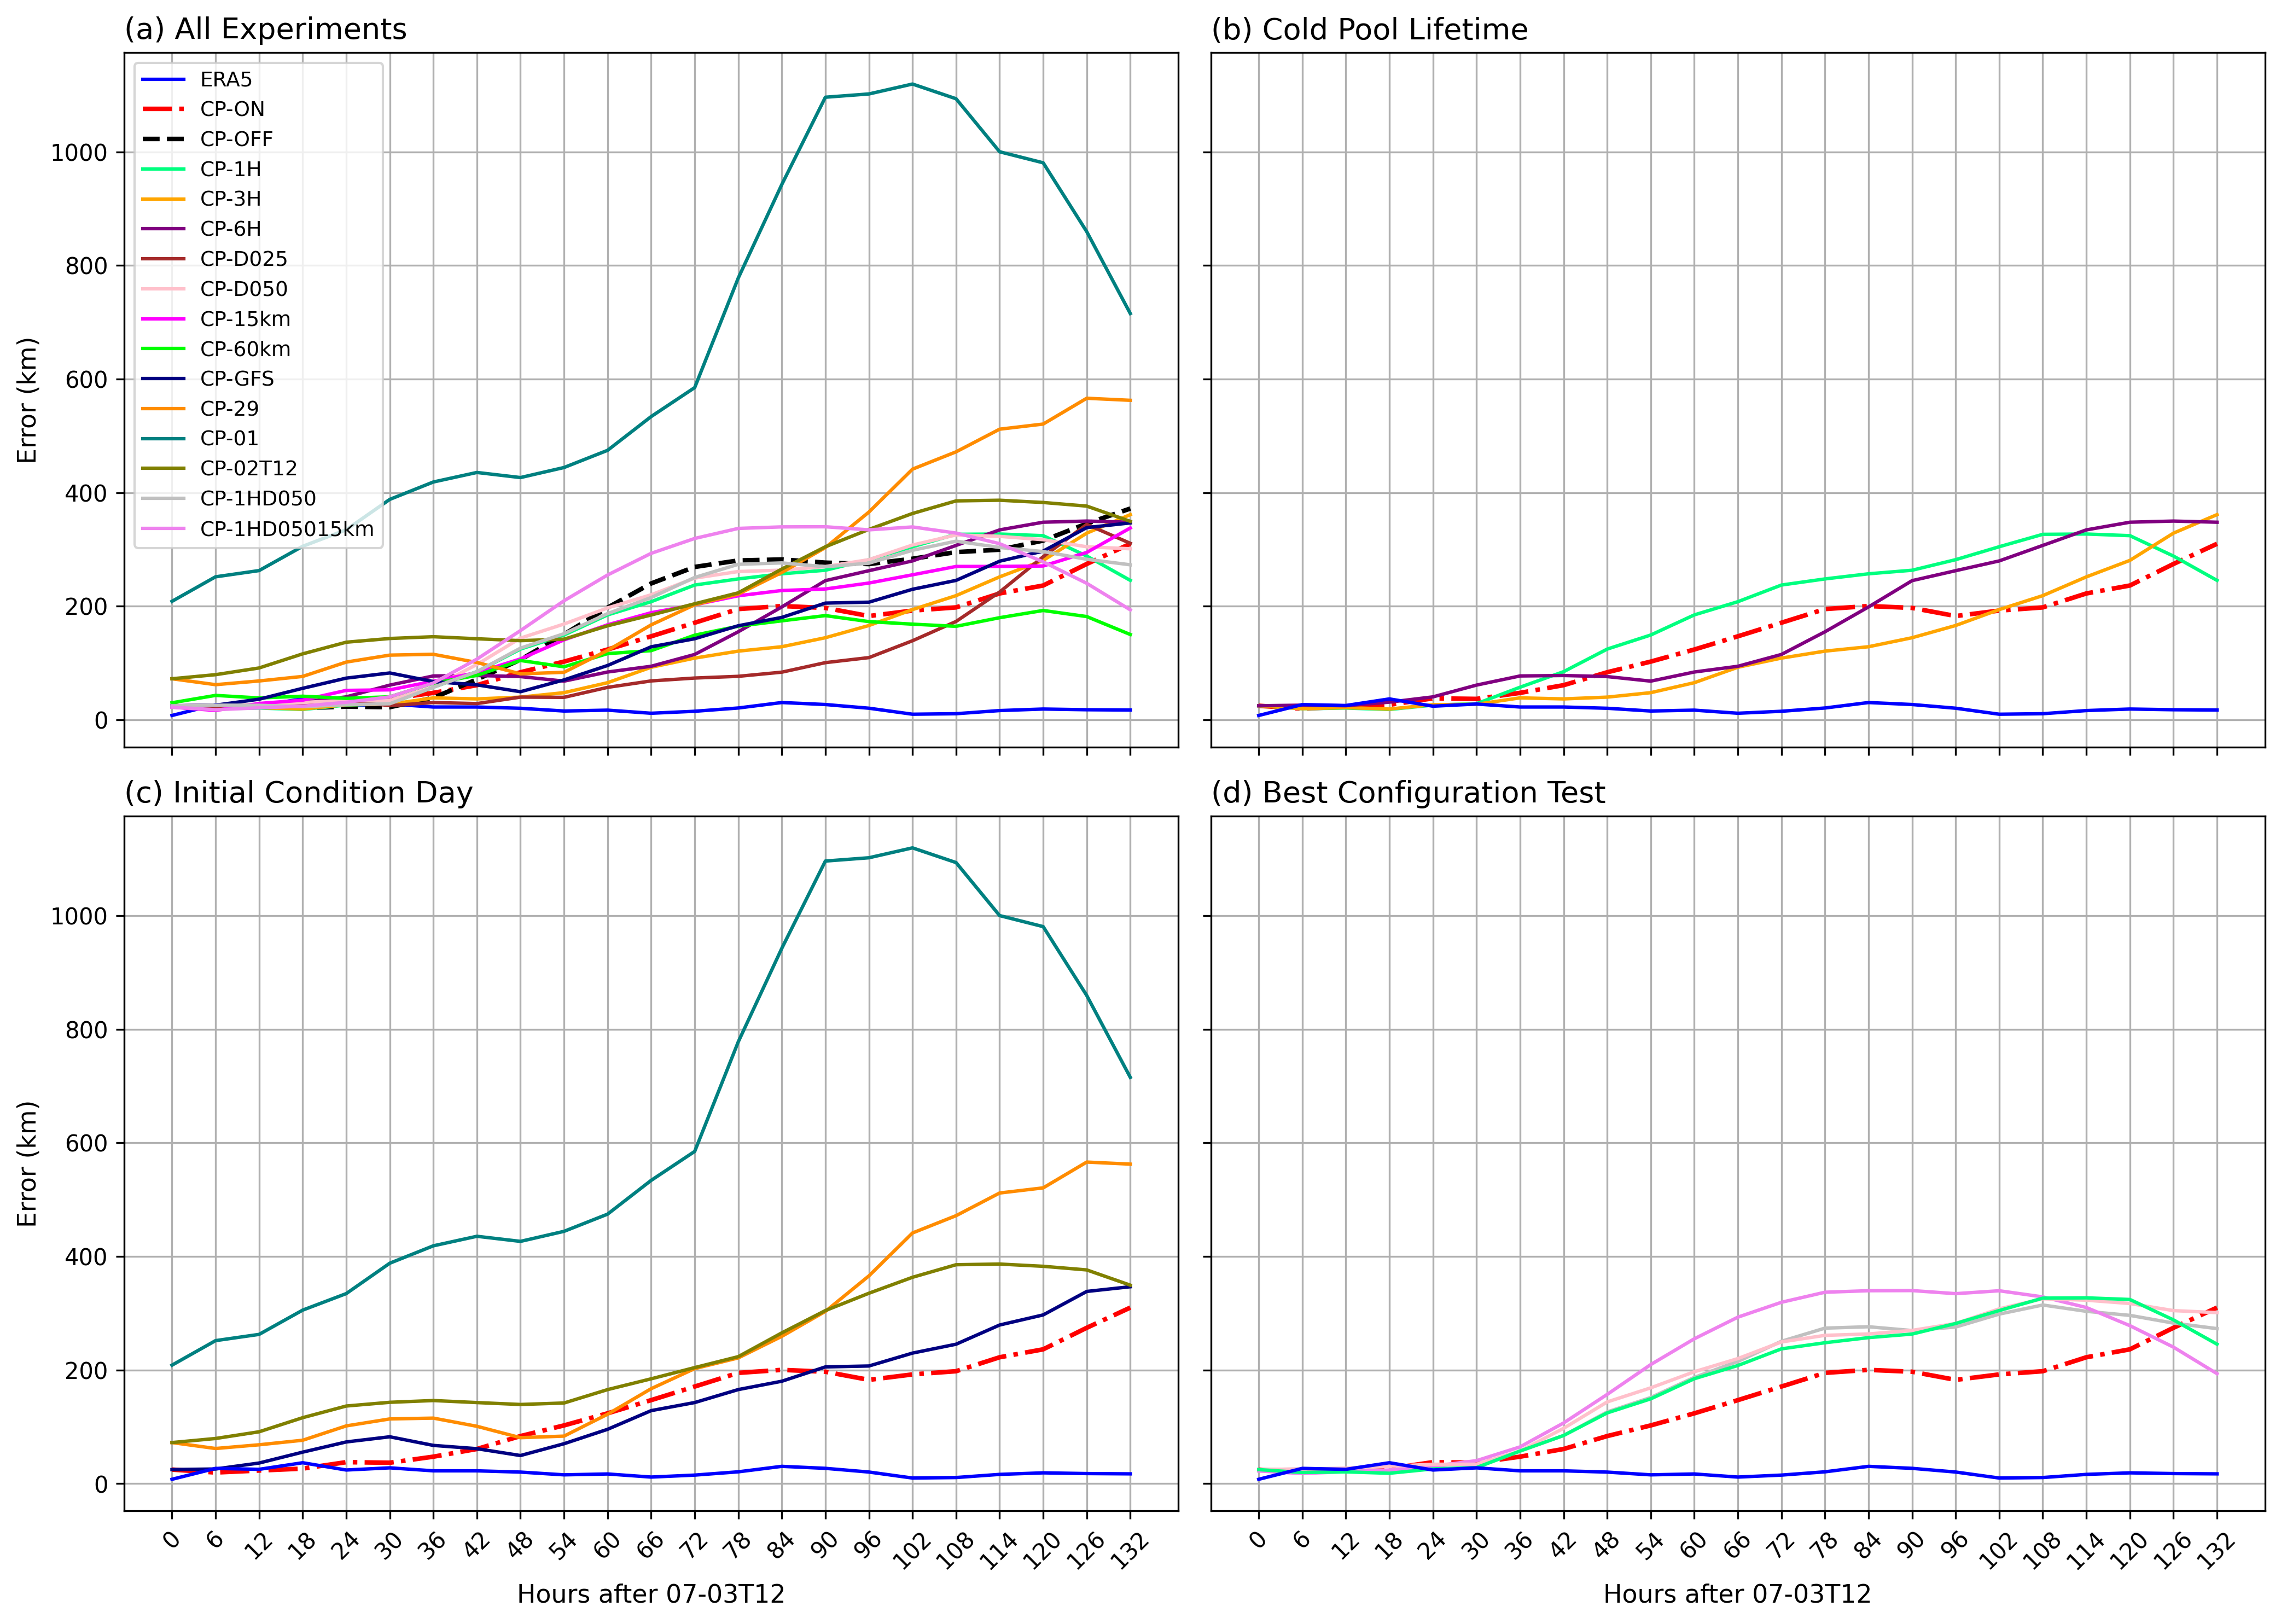
\includegraphics[width=\textwidth]{docs/figuras/chapter5/panel_2x2_error_comparison.png} % Substitua pelo caminho e extensão correta
    \vspace{0.5em}
    
    Source: Made by the author (2025). % Fonte abaixo da imagem
    \label{fig:panel_errors_before} % Label para referenciar no texto
\end{figure}

\pagebreak

It can be confirmed that CP-01 deviates significantly from the expected trajectory. Additionally, CP-6H offer limited discussion, as it is quite similar to the other experiments within their group. In Figure~\ref{fig:panel_errors_before} (d), CP-1HD05015km does not show a significant improvement and will consequently be withdrawn. We will retain CP-1HD050 to seek the effects related to this configuration in the context of other aspects of tropical cyclones.

To summarize the experiments we intend to keep, a new table has been created, similar to Table~\ref{tab:experiments_long}.

\pagebreak

\begin{table}[H]
	\centering
	\caption{Selected experiments}
	\label{tab:selected_experiments}
	\renewcommand{\arraystretch}{1.2}
	\resizebox{\textwidth}{!}{
		\begin{tabular}{
				>{\centering\arraybackslash}m{4cm}
				>{\centering\arraybackslash}m{9cm}
				>{\centering\arraybackslash}m{4cm}
			}
			\toprule
			Parameter & Description & ID \\
			\midrule
			
			Cold Pool Effect 
			& Turn on and off the cold pool parameterization scheme 
			& \makecell[l]{CP-ON\\CP-OFF (Control)} \\
			\midrule
			
			Initial Condition 
			& Compares the effect of two initial conditions, June 29, July 2nd (noon), and July 3rd. Tested with 1st July 
			& \makecell[l]{CP-29\\CP-02T12\\CP-03 (Control)} \\
			\midrule
			
			Cold Pool Lifetime 
			& Compares the effect of cold pool life time being 1h, 2h (default), 3h, and 6h 
			& \makecell[l]{CP-1H\\CP-2H (Control)\\CP-3H} \\
			\midrule
			
			Maximum Downdraft Height 
			& Compares the effect of the maximum downdraft height, being 0.25, 0.35, and 0.50 
			& \makecell[l]{CP-D025\\CP-D035 (Control)\\CP-D050} \\
			\midrule
			
			Resolution Experiment 
			& Evaluate the resolution effect on the results, degrading it into 60 km and enhancing it into 15 km 
			& \makecell[l]{CP-15km\\CP-30km (Control)\\CP-60km} \\
			\midrule
			
			Type of Initial Condition 
			& Changes the type of initial condition to be from the GFS model 
			& \makecell[l]{CP-ERA5 (Control)\\(CP-GFS)} \\
			\midrule
			
			Best Configuration Test 
			& A run with 2 changes inside the cold pool parameters 
			& CP-1HD050 \\
			\bottomrule
		\end{tabular}
	}
	
	\vspace{2mm}
	{\centering Source: Made by the author (2025).\par}
\end{table}


In the following subsection we will continue the results now keeping in mind the experiments listed at Table~\ref{tab:selected_experiments}.

%%%%%%%%%%%%%%%%%%%%%%%%%%%%%%%%%%%%%%%%%%

\subsection{Trajectory}


All trajectories are displayed in the Figure~\ref{fig:all_tracks_selected}. The trajectories of each group of the Table~\ref{tab:selected_experiments} can be found at Appendix B.

\begin{figure}[!ht]
    \centering
    \caption{All tracks with selected experiments from Table~\ref{tab:selected_experiments}} % Título acima da figura
    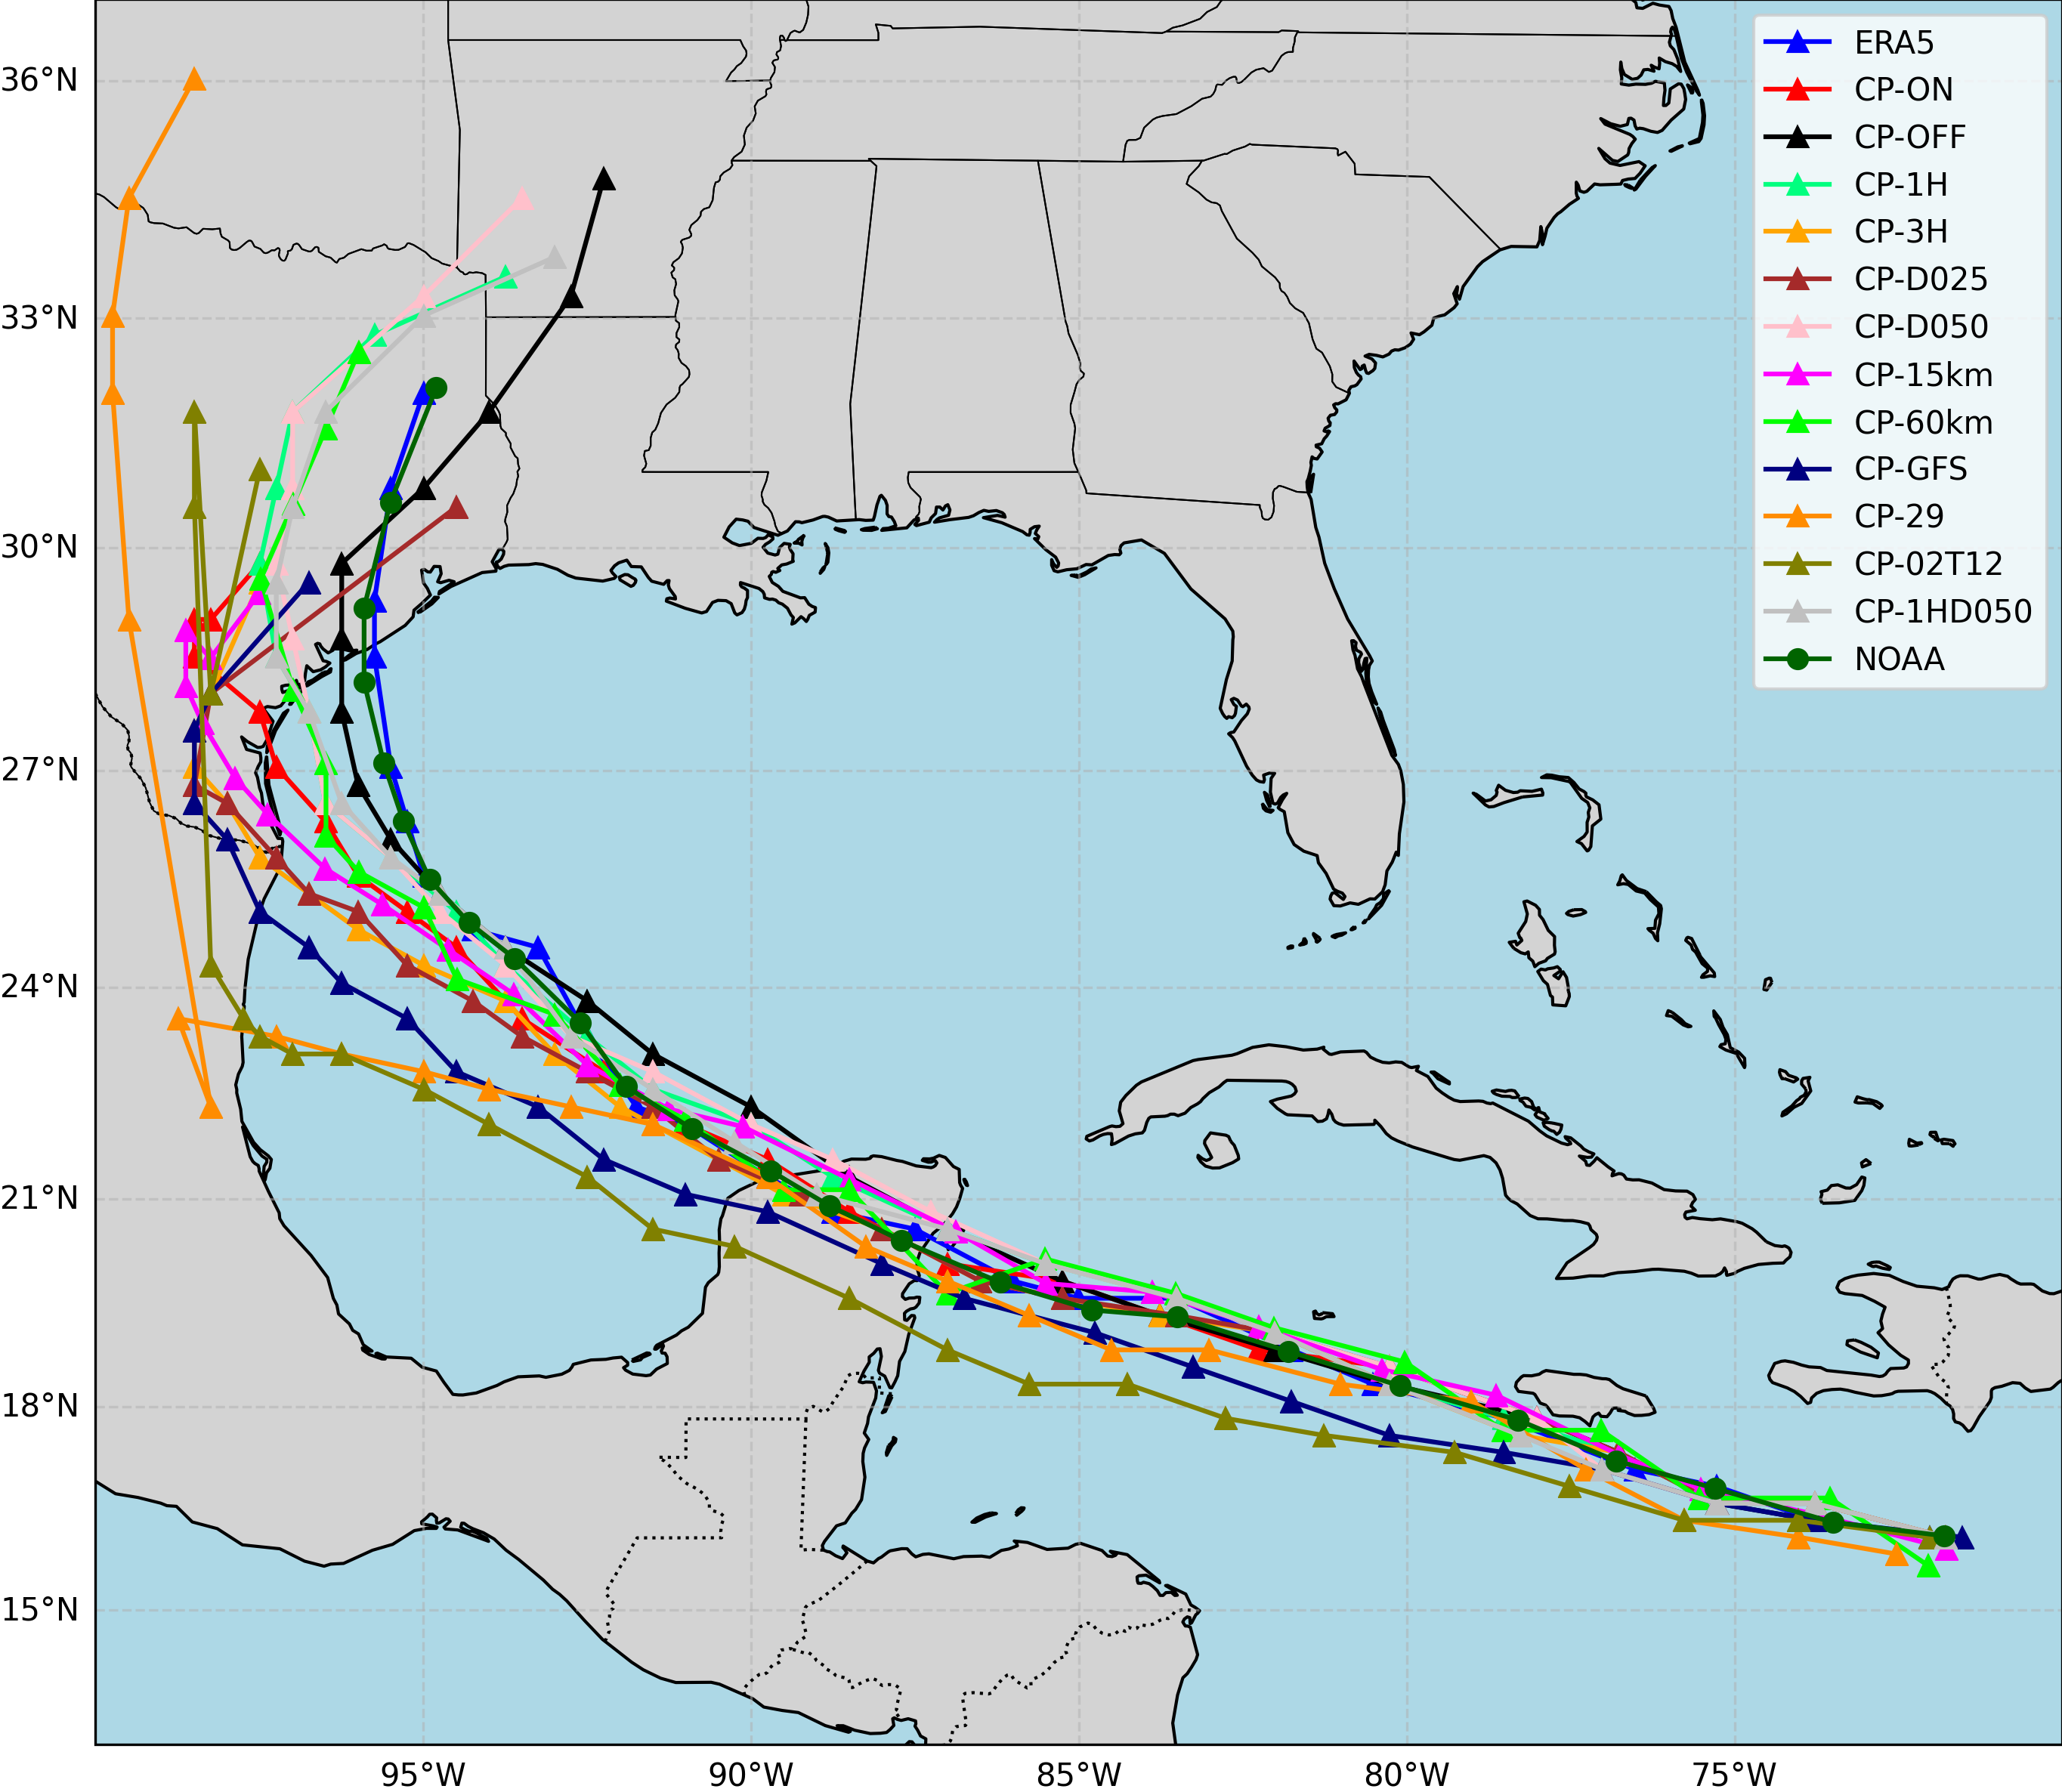
\includegraphics[width=\textwidth]{docs/figuras/chapter5/ALL_tracks_filter.png} 
    \vspace{0.5em}
    
    Source: Made by the author (2025). % Fonte abaixo da imagem
    \label{fig:all_tracks_selected} % Label para referenciar no texto
\end{figure}

This figure presents a map generated utilizing a tracking algorithm developed by the author. Firstly, the algorithm extracts each point corresponding to the minimum central pressure from the best track data between July 3rd and July 9th, 2024, sweeping a total integration period of 144 hours, with data plotted at 6-hour intervals. Furthermore, the minimum Mean Sea Level Pressure (MSLP) of the MONAN’s forecast and ERA5 reanalysis is extracted within a predefined spatial box surrounding the best track minimum central pressure. For instance, the initial bullet point depicted in dark green (representing NOAA’s best track at approximately 72.5° W) corresponds to the minimum central pressure obtained with the best track on July 3rd (00 UTC), 2024, while the final bullet point in dark green represents the data from July 9th (00 UTC), 2024 (close to 95° W).

At first glance, the reader will notice the observed congruence between the ERA5 reanalysis data and the best track observations. This strong agreement may be attributable to the reanalysis nature (Dulac et al., 2023), which integrates observational datasets throughout the integration period, thereby leading to this expected behaviour.

The CP-ON and CP-OFF experimental configurations exhibit comparable results for the majority of the integration period, with pronounced discrepancies evident near the Texas landfall and around the Yucatán Peninsula. A more detailed examination of these differences is warranted with other metrics. Concerning the cold pool lifetime, a 3-hour interval significantly deteriorates the accuracy of the forecasts. Furthermore, the downdraft maximum height coefficient of 0.50 appears to yield less precise results relative to the default values of 0.35 and 0.25. The trajectory forecasts utilizing a 60 km horizontal resolution demonstrate closer alignment with the reference data, outperforming the 15 km and 30 km horizontal resolutions, with the 60 km configuration exhibiting superior performance. Additionally, forecasts initialized with the GFS (CP-GFS) model appear to underperform in comparison to those initialized with ERA5.

It is observed that when initialization occurs before July 3rd (00 UTC), 2024, a visible degradation in trajectory forecast accuracy ensues. Note that there is a tendency for earlier initialization to result in poorer forecasts, a fact that can be confirmed later on with the MAE and RMSE metrics. This underscores the necessity of incorporating a module within the model to assess ensembles of initial conditions, also in agreement with what is found in the literature \cite{donkin2023capability}.

Finally, the configuration incorporating two parameters that have been changed simultaneously does not reveal significant deviations from the default setup. Overall, the forecasts exhibit a westward bias, a phenomenon that is also apparent in forecasts issued by the Hurricane Analysis and Forecast System (HAFS), as shown at Figure \ref{fig:berryl3rd}.

\begin{figure}[!ht]
	\centering
	\caption{Forecast made for Hurricane Beryl starting at July 3rd (00 UTC), 2024, available at the HAFS website} % Título acima da figura
	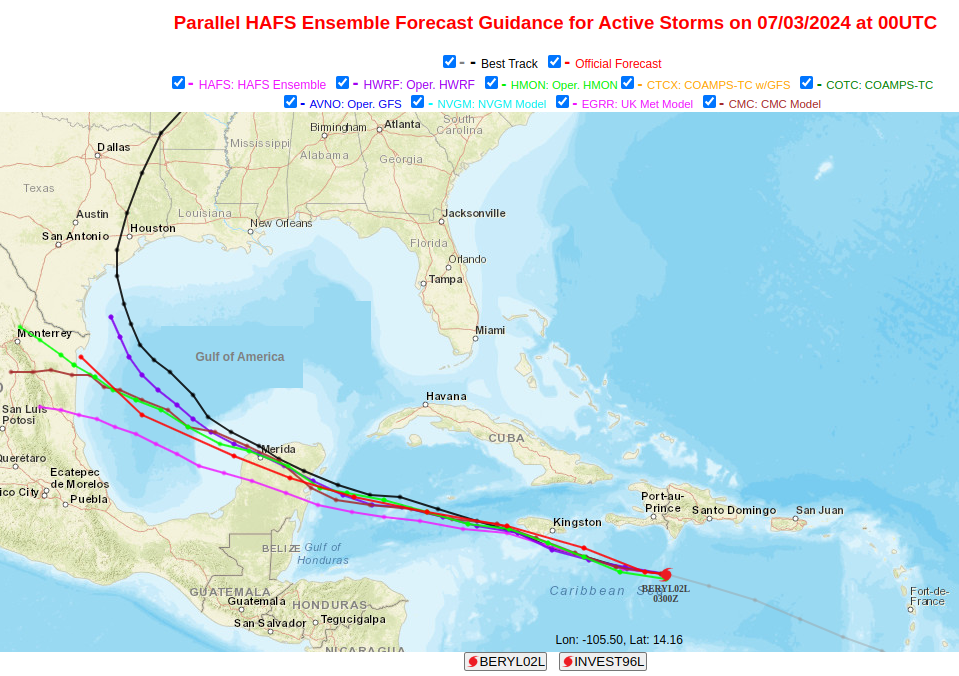
\includegraphics[width=\textwidth]{docs/figuras/chapter5/HAFS_trajectory.png} 
	\vspace{0.5em}
	Source: \url{https://www.emc.ncep.noaa.gov/HAFS/HAFSEPS/index.php} . % Fonte abaixo da imagem
	\label{fig:berryl3rd} % Label para referenciar no texto
\end{figure}

The next panel provides complementary information to the analysis, now in a more quantitative manner. It is important to mention that the time series display the errors after 12h of spin-up, and that value is maintained and the further analysis. In Figure (a), it is possible to better distinguish the differences among the experiments over time. In other words, it shows when each experiment presents lower errors throughout the integration period, along with an initial comparison among them. It is important to note that the vertical line E indicates the moment the hurricane makes landfall on the Yucatan Peninsula, while the vertical line F marks its entry into Texas. In Figure (b), this comparison becomes even clearer, especially because the bars are arranged vertically from the lowest to the highest error (from top to bottom).

\begin{figure}[!ht]
	\centering
	\caption{Track errors of the MONAN forecast and ERA5 reanalysis with the best track as reference. 12 hours of model spin-up are withdrawn from the analysis. (a) is displayed the distance error computed as the great circle, and (b), the MAE and RMSE calculated from (a).} % Título acima da figura
	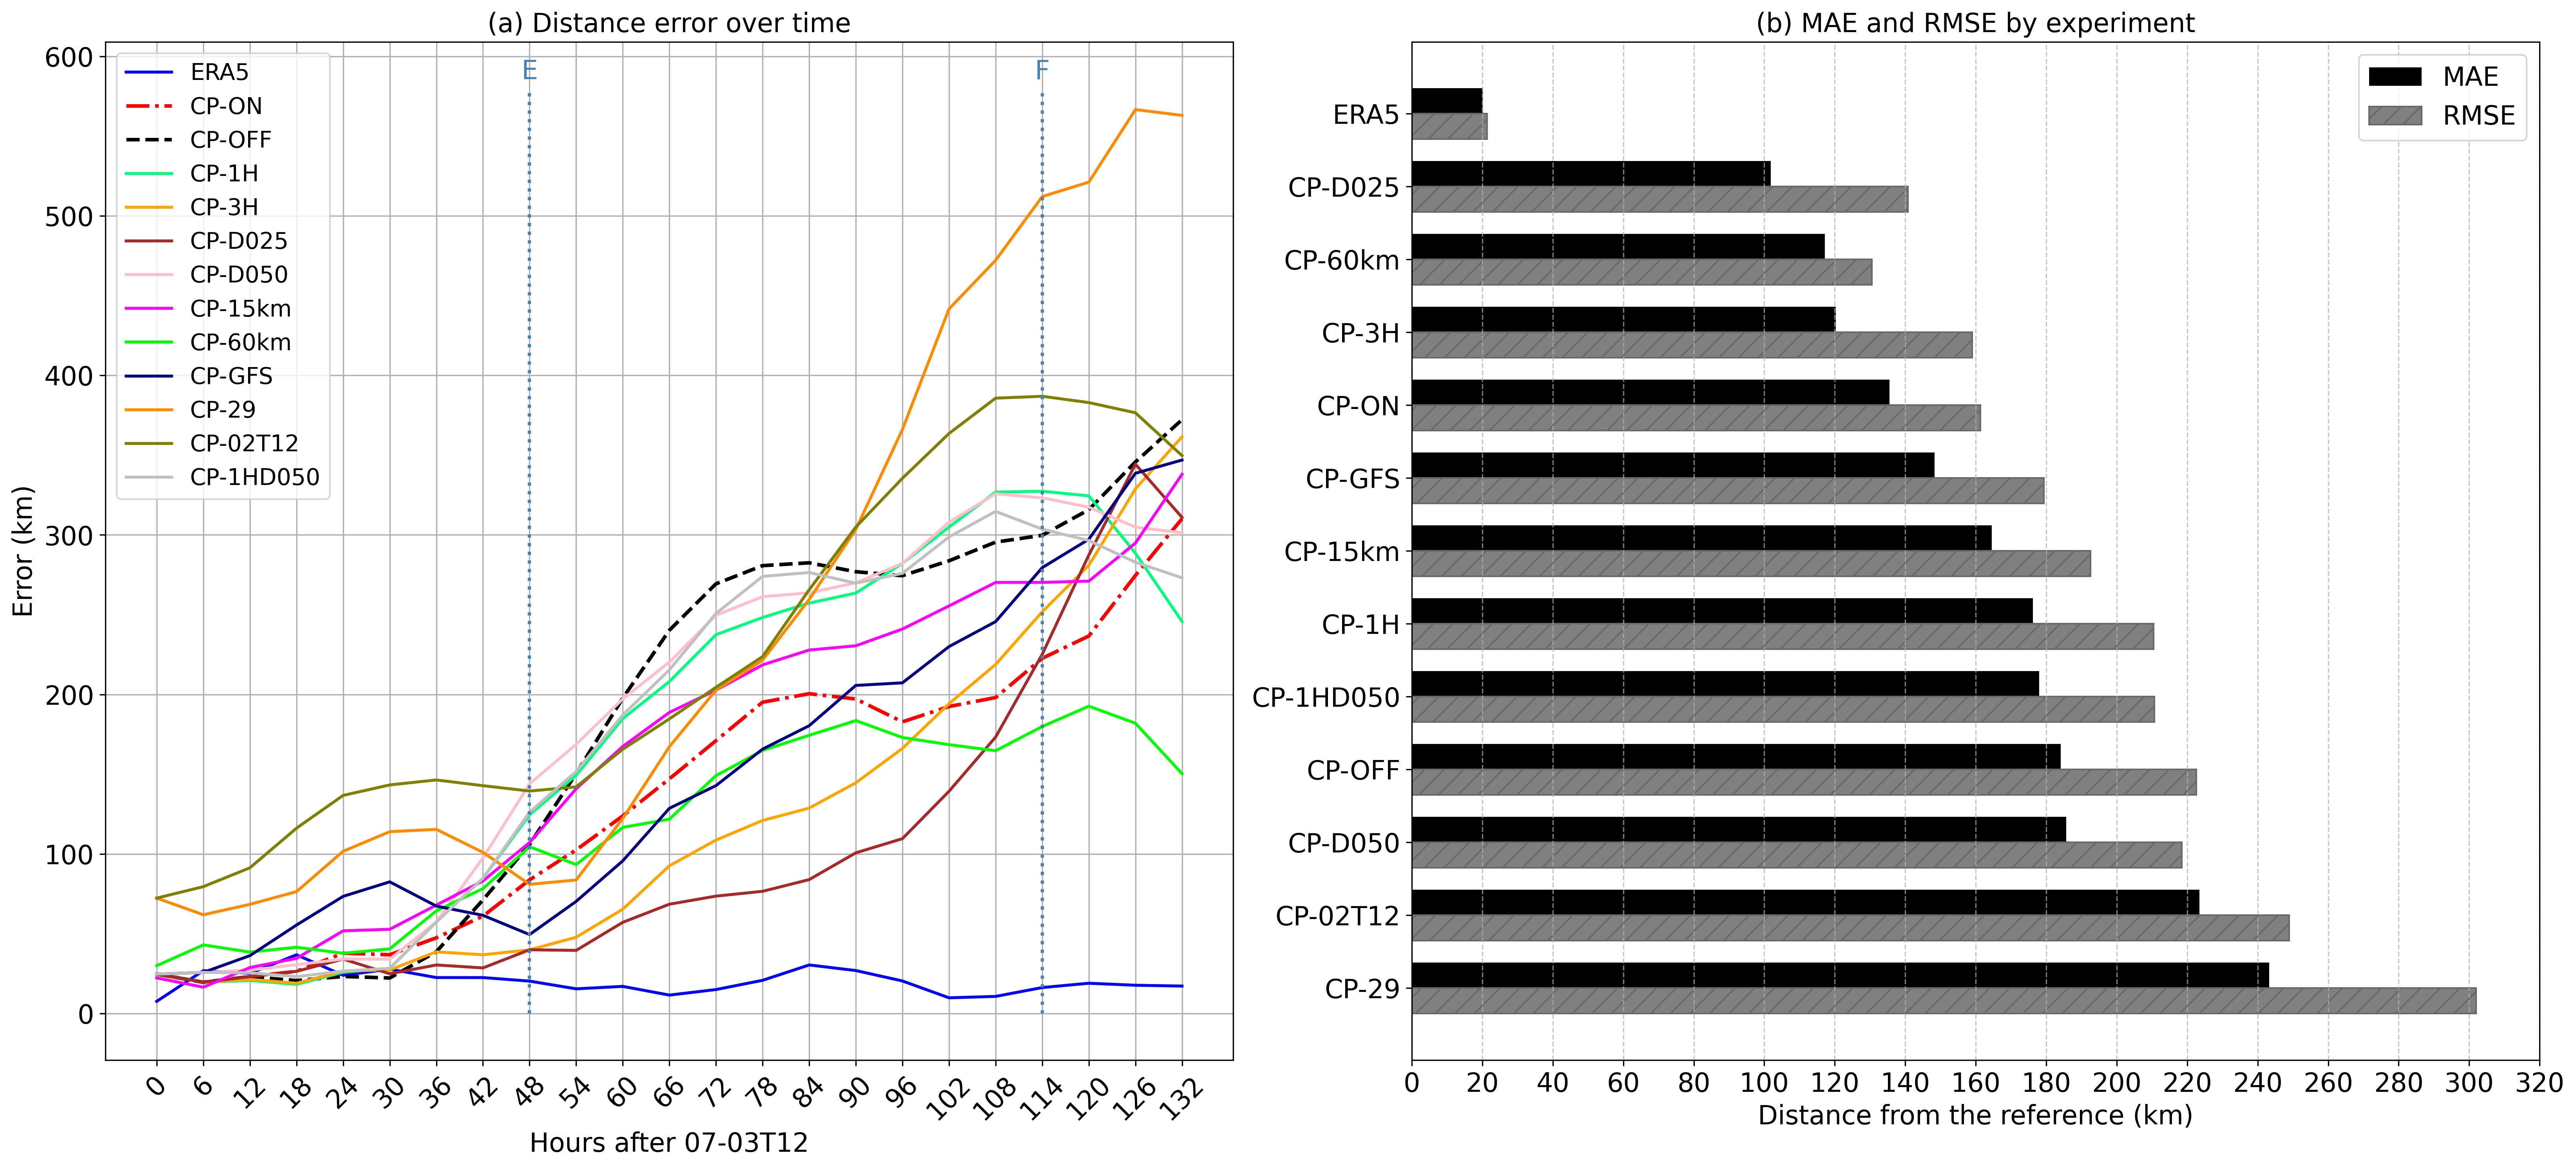
\includegraphics[width=\textwidth]{docs/figuras/chapter5/panel_errors_mae_rmse_FINAL.png} 
	\vspace{0.5em}
	Source: Made by the author, (2025).  % Fonte abaixo da imagem
	\label{fig:trackerrors} % Label para referenciar no texto
\end{figure}

As shown in the previous figure, ERA5 delivers the best track prediction performance. This could be attributed to the fact that ERA5 is a reanalysis product, meaning that observational data assimilation is injected into the model at each integration step. A fairer comparison would require conducting this analysis with another model similar to MONAN, which will be left for future work.

Overall, forecasts tend to show errors below 100 km up to 42 hours of lead time, except for those initialized earlier (CP-29 and CP-02T12). After 60 hours of forecast (two and a half days), some experiments begin to exceed 200 km of error. However, cold pool influence on track prediction only reaches this threshold after 84 hours (three and a half days), and the CP-D025 experiment only reaches it after about 111 hours (four and a half days). Therefore, we observe that with cold pool parameterization, forecast skill is extended by up to two days compared to the configuration without this scheme, for this specific case study.

In the literature, the best forecast limit reported is around 120 hours (five days) \cite{zhou2020prospects}, \cite{sippel2022impacts}. It is worth emphasizing that forecast errors beyond this threshold should be considered “chaotic,” given the nonlinear nature of the system.

The computation of MAE and RMSE provides insights into the overall error behavior in track forecasts. While MAE offers a generalized view of the error, RMSE takes into account the squared deviations, assigning more weight to larger errors at each time step. In general, it is notable that simply enabling the cold pool parameterization (CP-ON) already improved the track forecast, reducing the MAE by approximately 22\% compared to CP-OFF. Furthermore, we observe that tuning the parameters, such as in CP-D025, CP-3H, and modifying the resolution to 60 km (CP-60km), further enhanced this performance.

By observing the Figure \ref{fig:berryl3rd} and Figure \ref{fig:trackerrors}, one could notice the westward deviation in the forecast. The next panel showing the CTE and ATE can confirm this behaviour, at Figure \ref{fig:cte}.

\begin{figure}[!ht]
	\centering
	\caption{CTE (a) and ATE (b).} % Título acima da figura
	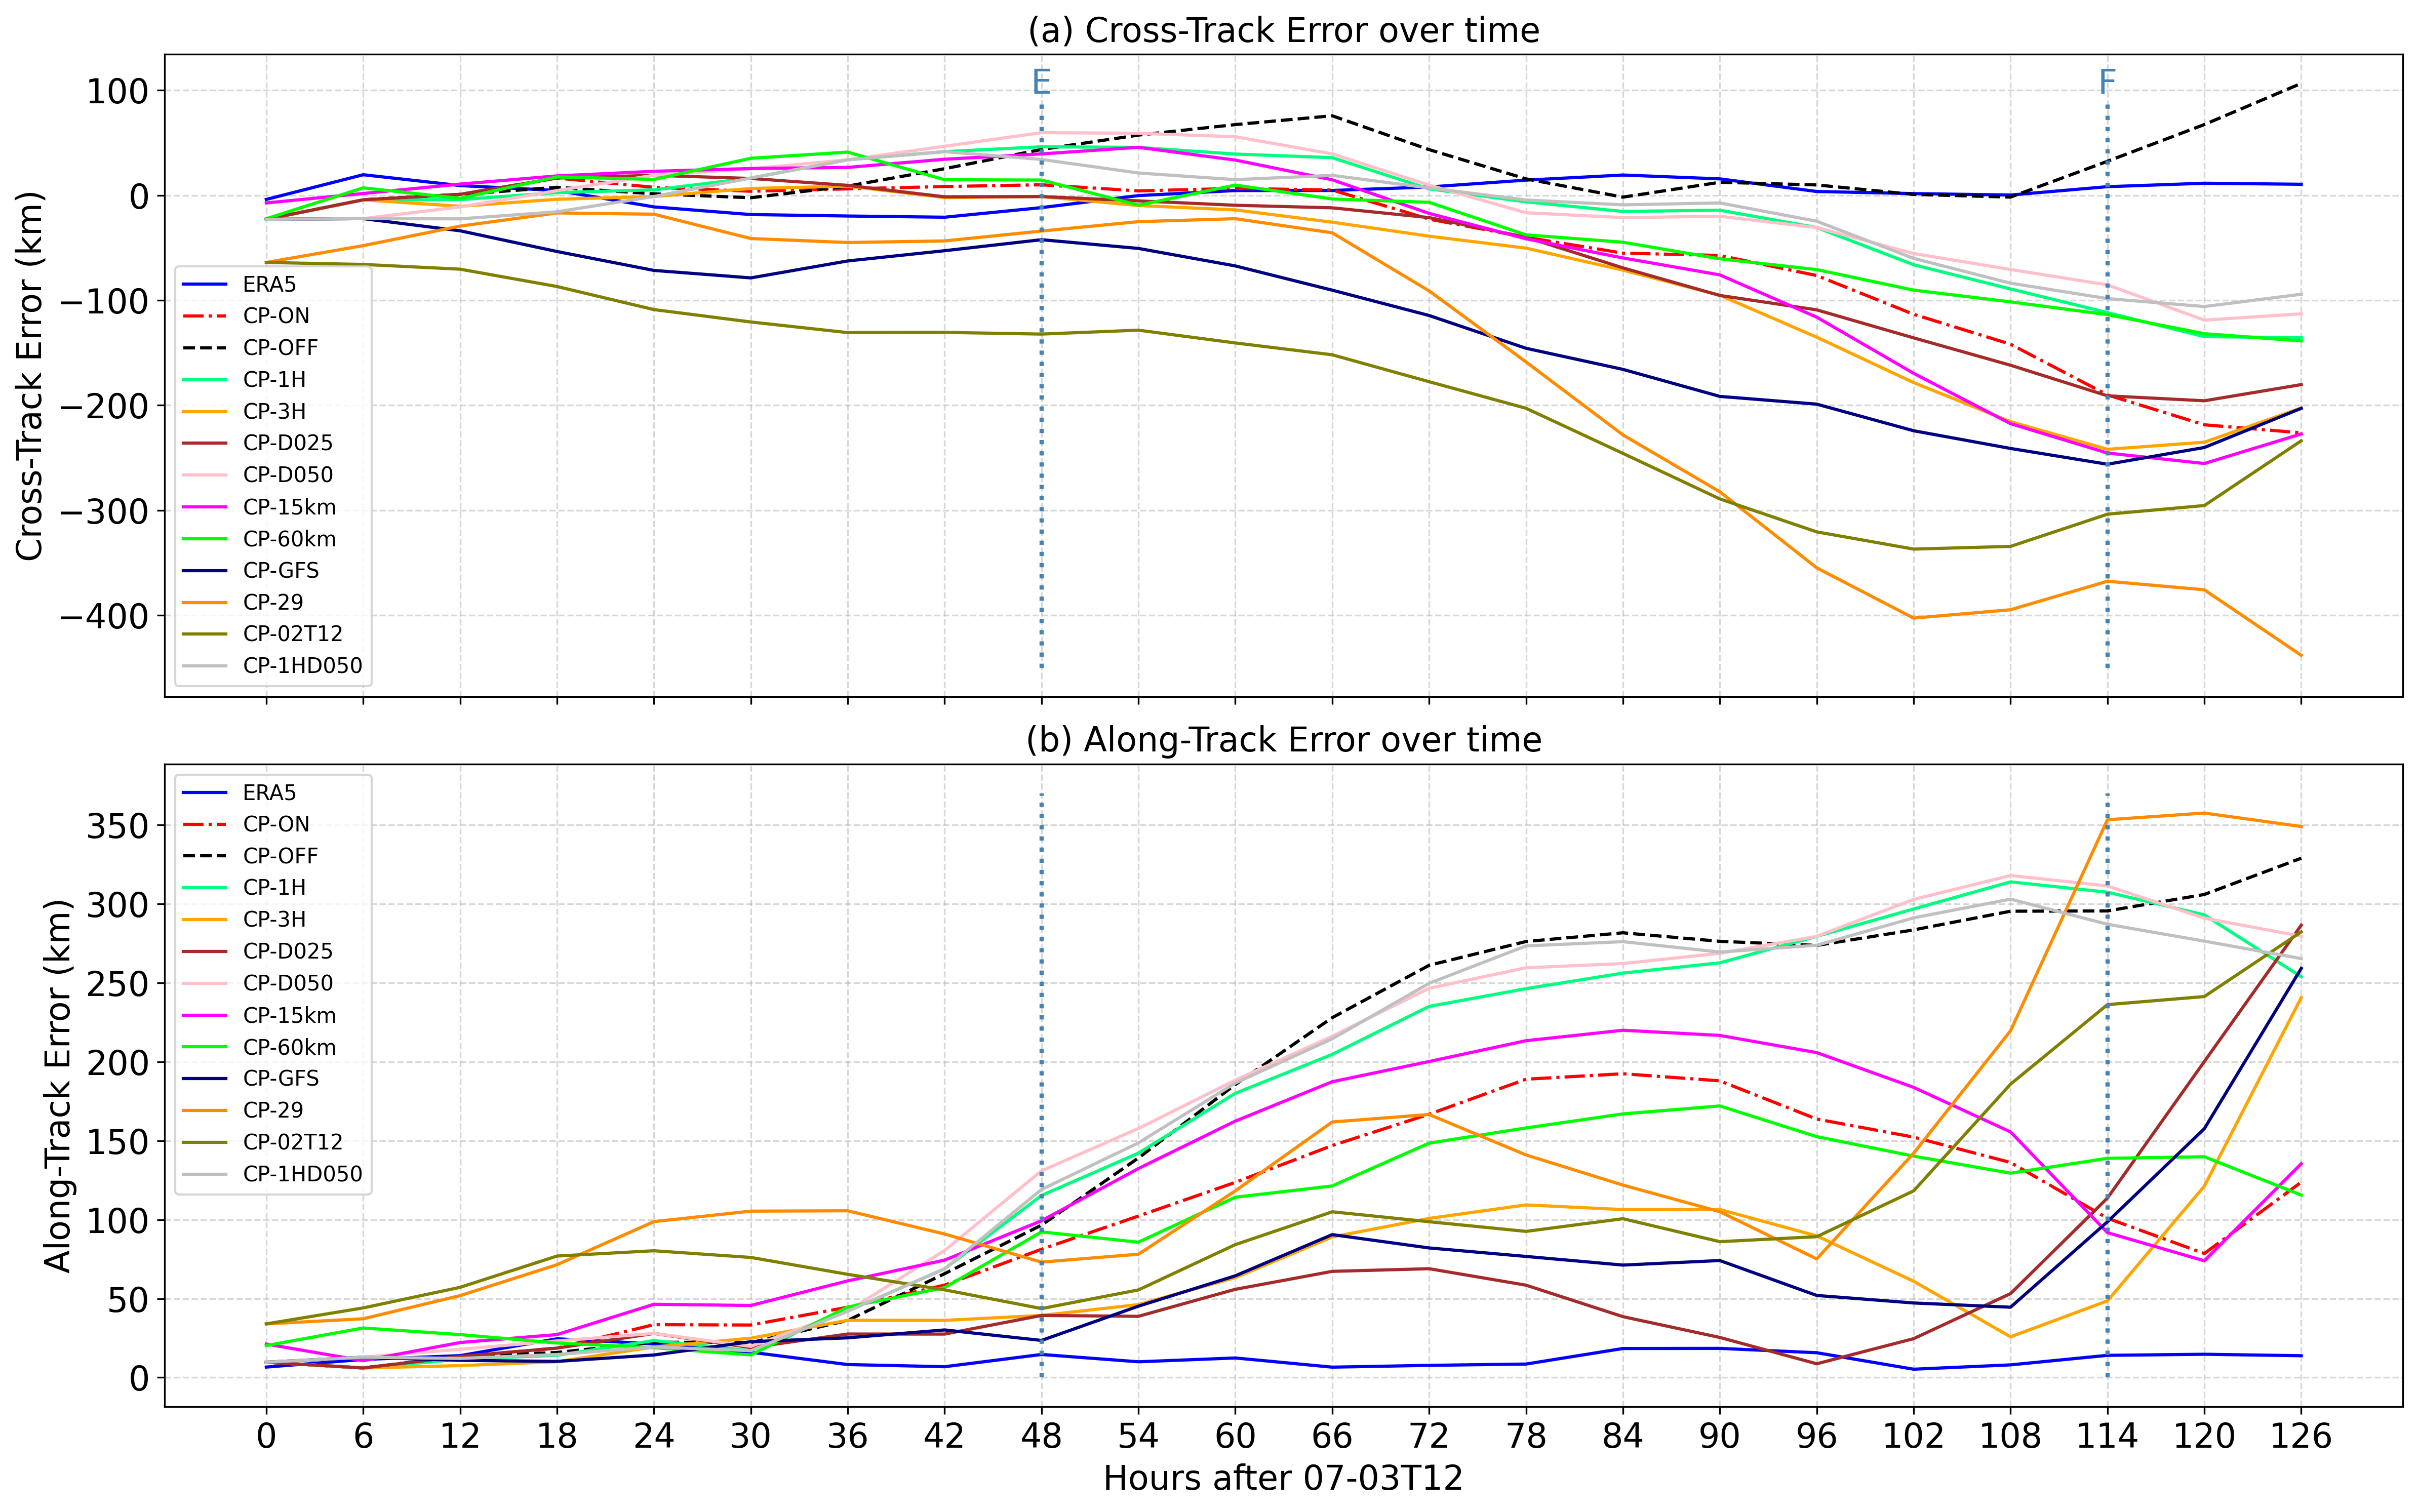
\includegraphics[width=\textwidth]{docs/figuras/chapter5/Cross_Track_Along_Track_Errors_FINAL.png} 
	\vspace{0.5em}
	Source: Made by the author, (2025).  % Fonte abaixo da imagem
	\label{fig:cte} % Label para referenciar no texto
\end{figure}

Overall, most of the forecasts show a negative CTE, meaning there is a leftward (westward) deviation from the observed trajectory, confirming Figure \ref{fig:all_tracks_selected}, which displays all the tracks, and Figure \ref{fig:berryl3rd}. This trend is particularly clear in the CP-02T12 experiment. Since the first hour of the forecast, the CTE is negative, which aligns with the fact that the predicted trajectory is consistently to the left of the observed one.

It is interesting to note that the CTE behavior differs significantly between the CP-ON and CP-OFF experiments. While CP-OFF maintains a positive CTE, CP-ON gradually shifts to a negative CTE as the integration period progresses. Notably, CP-ON begins to deviate leftward after around 72 hours of integration, after passing through the Yucatan Peninsula, whereas in other experiments, such as CP-OFF and CP-D025, this deviation occurs earlier.

Interestingly, despite exhibiting large overall errors (Figure \ref{fig:trackerrors}), the CP-D050 experiment performs better than CP-ON in this metric, as it does not deviate as strongly. This highlights the importance of evaluating forecast performance from multiple perspectives and understanding the sources of these differences, which we will further investigate using meteorological fields.

This westward bias was also noted in the forecasts from both the HAFS (Figure \ref{fig:berryl3rd}) and the UK Met Office  (Figure \ref{fig:metoff}) for Hurricane Beryl.

\begin{figure}[!ht]
	\centering
	\caption{Tracking available by the UK Met Office.} % Título acima da figura
	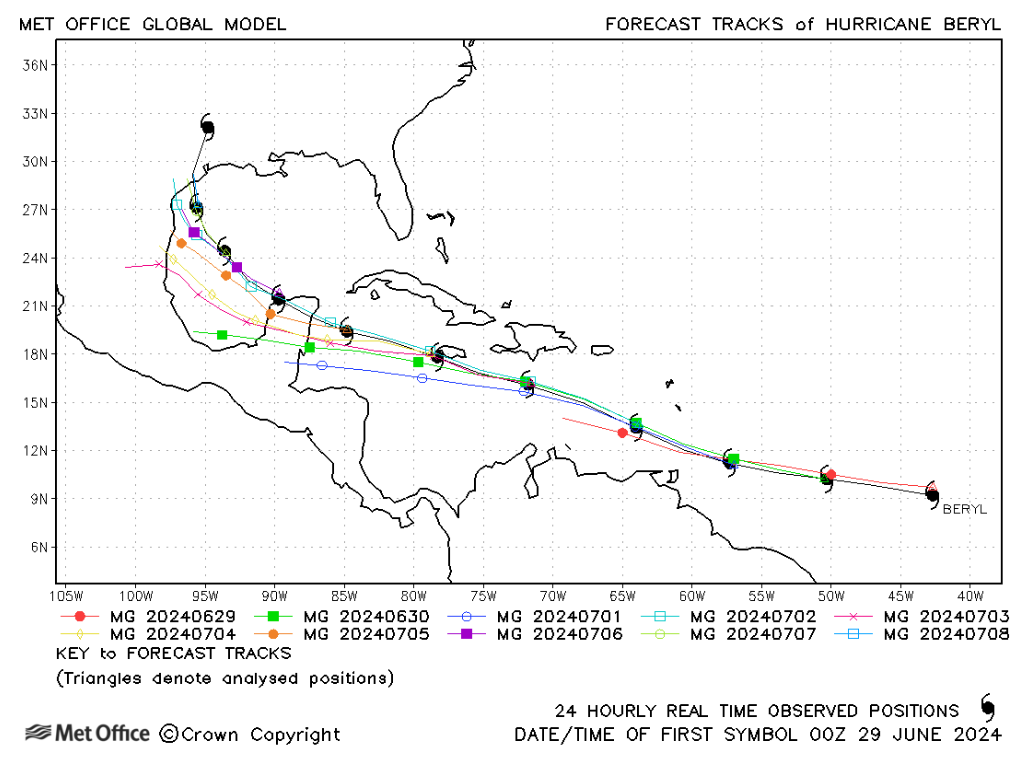
\includegraphics[width=\textwidth]{docs/figuras/chapter5/MetOffice.png} 
	\vspace{0.5em}
	Source: \url{https://www.metoffice.gov.uk/research/weather/tropical-cyclones/verification/seasons/nhem2024.}  % Fonte abaixo da imagem
	\label{fig:metoff} % Label para referenciar no texto
\end{figure}

The report \cite{metoffice2024} indicates that the track was forecasted with a notable degree of accuracy throughout the Caribbean region, furthermore, it was observed that there was a left-of-track bias in the forecasts as Beryl progressed into the Gulf of Mexico.

In general, the ATE is positive across all experiments, indicating a consistent tendency for the MONAN model to move faster than observed. Note that ERA5 also displays this trend, though it is not as pronounced as in MONAN.

When comparing CP-ON and CP-OFF, a growing ATE trend is evident in CP-OFF. As the integration period increases, CP-OFF moves increasingly ahead of the observed track, reaching 225 km ahead at 66 hours, whereas CP-ON is only about 150 km ahead at the same time.

The CP-D025 experiment appears to be more in phase with the observations in this metric than CP-ON during most of the forecast period, despite having a greater leftward deviation compared to CP-ON. Despite larger errors in track positioning, the early-initialized forecasts manage to better match the best track in terms of propagation speed. In this case, the forecast initialized with GFS outperformed the forecast initialized with ERA5 during most of the integration period.

A mean error performance of all MONAN forecasts were computed and shown at Figure \ref{fig:monera5}.

\begin{figure}[!ht]
	\centering
	\caption{Overall performance of MONAN trajectory forecasts compared with ERA5 reanalysis.} % Título acima da figura
	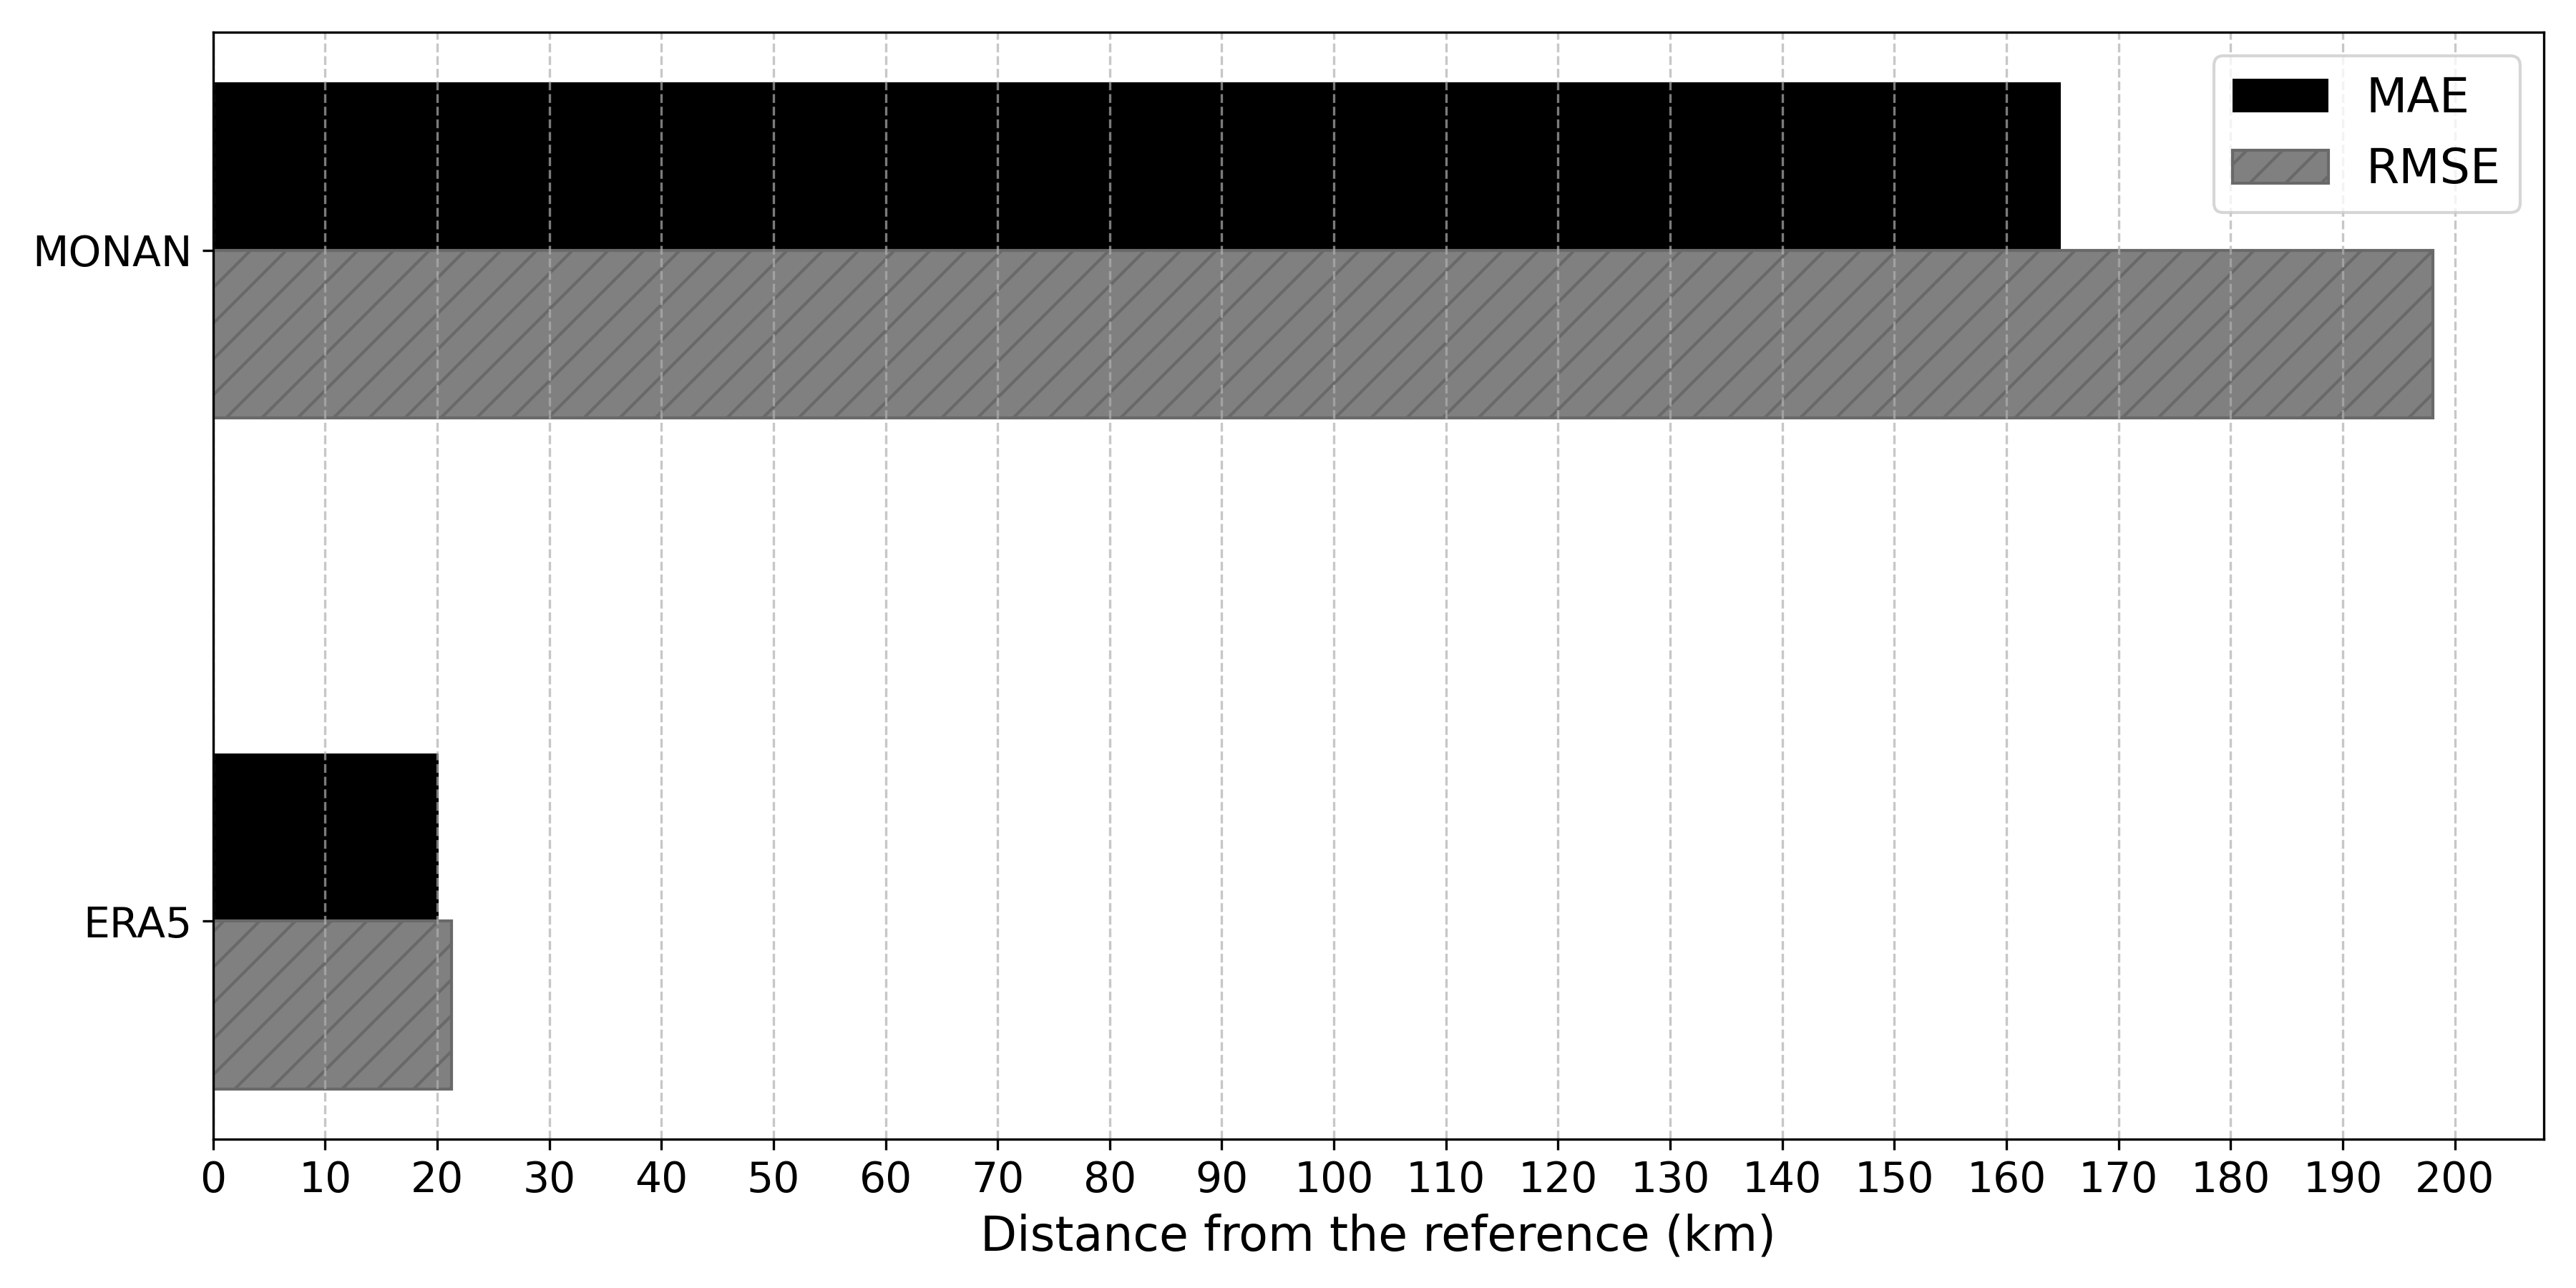
\includegraphics[width=\textwidth]{docs/figuras/chapter5/barplot_monan_vs_era5_mae_rmse_FINAL.png} 
	\vspace{0.5em}
	Source: Made by the author (2025).  % Fonte abaixo da imagem
	\label{fig:monera5} % Label para referenciar no texto
\end{figure}

In general, the MONAN forecast is approximately 8 times greater than the ERA5 reanalysis. Again, we can infer that it is not a fair comparison between the MONAN forecast and the ERA5 reanalysis, but it is important to notice the error scale to give us insights about improving the MONAN forecast.




\subsection{Intensity}




\subsection{Rainfall}

\subsubsection{Pattern and spatial rainfall distribution}

\subsubsection{Rainfall mean and overall distribution}

\subsubsection{MONAN performance at forecasting rainfall}

\subsection{Discussion of key outcomes}

